%
% Template Laporan Skripsi/Thesis Universitas Indonesia
%
% @author  Ichlasul Affan, Azhar Kurnia
% @version 2.2.1
%
% Dokumen ini dibuat berdasarkan standar IEEE dalam membuat class untuk
% LaTeX dan konfigurasi LaTeX yang digunakan Fahrurrozi Rahman ketika
% membuat laporan skripsi, yang kemudian diadaptasi oleh Andreas Febrian dan
% Lia Sadita untuk template skripsi tahun 2010.
% Konfigurasi template sebelumnya telah disesuaikan dengan
% aturan penulisan thesis yang dikeluarkan UI pada tahun 2017.
%


%
% Tipe dokumen adalah report dengan satu kolom.
%
\documentclass[12pt, a4paper, onecolumn, twoside, final]{report}
\raggedbottom

% Load konfigurasi LaTeX untuk tipe laporan thesis
\usepackage{_internals/uithesis}
%
\UseRawInputEncoding
% Load konfigurasi khusus untuk laporan yang sedang dibuat
%-----------------------------------------------------------------------------%
% Judul Dokumen
%-----------------------------------------------------------------------------%
%
% Judul laporan.
\def\judul{Judul Karya Ilmiah Anda}
%
% Tulis kembali judul laporan namun dengan bahasa Ingris
\def\judulInggris{Your Scientific Publication Title}


%-----------------------------------------------------------------------------%
% Tipe Dokumen
%-----------------------------------------------------------------------------%
%
% Tipe laporan, dapat berisi: Laporan Kerja Praktik, Kampus Merdeka, Skripsi, Tugas Akhir, Thesis, atau Disertasi
\def\type{Skripsi}
%
% Nama jalur Kampus Merdeka (hanya perlu diisi jika tipe laporan adalah Kampus Merdeka
% Contoh isian (khusus Fasilkom): Studi Independen, Magang Mitra, Magang BUMN, Bangkit, Apple Academy, BYOC
\def\kampusMerdekaType{}
% Jika ada perwakilan mitra, isi dengan jabatan perwakilan mitra tersebut
% (misal: Cohort Manager)
% Kosongkan jika tidak ada perwakilan mitra
\def\partnerPosition{}
% Jika ada perwakilan mitra, isi dengan nama perusahaan atau nama program
% (misal: PT. Astra International, Bangkit Academy 2023)
% Kosongkan jika tidak ada perwakilan mitra
\def\partnerInstance{}
%
% Jenjang studi, dapat berisi: Diploma, Sarjana, Magister, atau Doktor
\def\jenjang{Sarjana}


%-----------------------------------------------------------------------------%
% Informasi Penulis
%-----------------------------------------------------------------------------%
%
% Tulis nama Anda
% Kosongkan penulisDua dan penulisTiga jika Anda melaksanakan tugas akhir/laporan secara individu
\def\penulisSatu{Nama Lengkap Anda 1} % nama lengkap penulis pertama
\def\penulisDua{} % nama lengkap penulis kedua
\def\penulisTiga{} % nama lengkap penulis ketiga
%
% Tulis NPM Anda
% Kosongkan npmDua dan npmTiga jika Anda melaksanakan tugas akhir/laporan secara individu
\def\npmSatu{Nomor Anda 1} % NPM penulis pertama
\def\npmDua{} % NPM penulis kedua
\def\npmTiga{} % NPM penulis ketiga
%
% Tulis Program Studi yang Anda ambil
% Kosongkan programDua dan programTiga jika Anda melaksanakan tugas akhir/laporan secara individu
\def\programSatu{Jurusan Anda 1} % program studi penulis pertama
\def\programDua{} % program studi penulis kedua
\def\programTiga{} % program studi penulis ketiga
%
% Tulis Program Studi yang Anda ambil dalam bahasa inggris
% Kosongkan programDua dan programTiga jika Anda melaksanakan tugas akhir/laporan secara individu
\def\studyProgramSatu{Your study program 1} % 1st author's study program
\def\studyProgramDua{} % 2nd author's study program
\def\studyProgramTiga{} % 3rd author's study program


%-----------------------------------------------------------------------------%
% Informasi Dosen Pembimbing & Penguji
%-----------------------------------------------------------------------------%
%
% Tuliskan pembimbing
% Untuk Kampus Merdeka: Tuliskan dosen PIC/pembimbing dari Fakultas Anda
\def\pembimbingSatu{Pembimbing Pertama Anda}
% S1 s.d. S3: Kosongkan jika tidak ada pembimbing kedua
% Untuk Kampus Merdeka: Tuliskan penanggung jawab/penyelia/mitra
%                       dari program Kampus Merdeka yang Anda ambil (jika ada)
\def\pembimbingDua{}
% S2 & S3: Kosongkan jika tidak ada pembimbing ketiga
\def\pembimbingTiga{}

%
% Tuliskan penguji
\def\pengujiSatu{Penguji Pertama Anda}
\def\pengujiDua{Penguji Kedua Anda}
% Kosongkan jika tidak ada penguji ketiga (umumnya penguji ketiga hanya ada untuk S2)
\def\pengujiTiga{}
% Kosongkan jika tidak ada penguji keempat, kelima, atau keenam (umumnya penguji > 3 hanya ada untuk S3)
\def\pengujiEmpat{}
\def\pengujiLima{}
\def\pengujiEnam{}


%-----------------------------------------------------------------------------%
% Informasi Lain (Asal Fakultas, Tanggal, dsb.)
%-----------------------------------------------------------------------------%
%
% Tuliskan Fakultas dimana penulis berada
\def\fakultas{Fakultas Anda}
%
% Tuliskan bulan dan tahun publikasi laporan
\Var{\bulanTahun}{Bulan Tahun}
%
% Tuliskan gelar yang akan diperoleh dengan menyerahkan laporan ini
\def\gelar{Gelar Jurusan Anda}
%
% Tuliskan tanggal pengesahan laporan, waktu dimana laporan diserahkan ke
% penguji/sekretariat
\def\tanggalSiapSidang{Tanggal Bulan Tahun}
%
% Tuliskan tanggal keputusan sidang dikeluarkan dan penulis dinyatakan
% lulus/tidak lulus
\def\tanggalLulus{Tanggal Bulan Tahun}


%-----------------------------------------------------------------------------%
% Judul Setiap Bab
%-----------------------------------------------------------------------------%
%
% Berikut ada judul-judul setiap bab.
% Silahkan diubah sesuai dengan kebutuhan.
%
\Var{\kataPengantar}{Kata Pengantar}
\Var{\babSatu}{Pendahuluan}
\Var{\babDua}{Kerangka Berpikir}
\Var{\babTiga}{Penggunaan Lanjutan}
\Var{\babEmpat}{Struktur Template}
\Var{\babLima}{Kasus-Kasus Khusus}
\Var{\kesimpulan}{Penutup}


%-----------------------------------------------------------------------------%
% Capitalized Variables
% Anda tidak perlu mengubah apapun di bagian ini
%-----------------------------------------------------------------------------%
\Var{\Judul}{\judul}
\Var{\Type}{\type}
\Var{\PenulisSatu}{\penulisSatu}
\Var{\PenulisDua}{\penulisDua}
\Var{\PenulisTiga}{\penulisTiga}
\Var{\Fakultas}{\fakultas}
\Var{\ProgramSatu}{\programSatu}
\Var{\ProgramDua}{\programDua}
\Var{\ProgramTiga}{\programTiga}



% Daftar pemenggalan suku kata dan istilah dalam LaTeX
%
% Hyphenation untuk Indonesia
%
% @author  Andreas Febrian
% @version 2.1.2
% @edit by Ichlasul Affan, Muhammad Aulia Adil Murtito
%
% Tambahkan cara pemenggalan kata-kata yang salah dipenggal secara otomatis
% oleh LaTeX. Jika kata tersebut dapat dipenggal dengan benar, maka tidak
% perlu ditambahkan dalam berkas ini. Tanda pemenggalan kata menggunakan
% tanda '-'; contoh:
% menarik
%   --> pemenggalan: me-na-rik
%


% Silakan ganti ke bahasa Inggris (\selectlanguage{english}) jika Anda merasa terlalu banyak kata bahasa Inggris yang pemenggalannya tidak benar.
%\selectlanguage{english}


\hyphenation{
    % alphabhet A
    a-na-li-sa an-da a-tur a-tur-an
    a-pli-ka-si
    % alphabhet B
    bab ba-ngun-an
    be-be-ra-pa
    ber-fung-si
    ber-ge-rak
    ber-ke-lan-jut-an
    ber-o-per-ra-si
    ber-pe-nga-ruh
    bi-sa
    % alphabhet C
    ca-ri Com-po-nent-UML
    % alphabhet D
    di-da-pat-kan di-sim-pan di-pim-pin di-tam-bah-kan di-tem-pat-kan de-ngan da-e-rah di-ba-ngun di-gu-na-kan da-pat di-nya-ta-kan
    di-se-mat-kan di-sim-bol-kan di-pi-lih di-li-hat de-fi-ni-si di-de-fi-ni-si-kan di-mo-del-kan di-mi-li-ki di-re-a-li-sa-si-kan di-su-sun
    % alphabhet E
    eks-pli-sit e-ner-gi en-gi-neer en-gi-neer-ing eks-klu-sif ele-men
    % alphabhet F
    fa-si-li-tas
    fung-si fung-si-nya
    % alphabhet G
    ga-bung-an ge-rak ge-ne-ral ge-ne-ra-li-sa-si
    % alphabhet H
    ha-la-man
    ha-lang-an
    % alphabhet I
    in-fra-struk-tur i-ni-si-a-si
    % alphabhet J
    % alphabhet K
    ke-hi-lang-an
    ke-ter-hu-bung-an
    ku-ning
    kua-li-tas ka-me-ra ke-mung-kin-an ke-se-pa-ham-an
    ke-ti-dak-se-su-ai-an
    % alphabhet L
    ling-kung-an
    % alphabhet M
    ma-na-je-men me-neng-ah meng-a-da-kan me-mo-ni-tor
    me-mer-lu-kan me-mo-del-kan men-de-fi-ni-si-kan men-ja-di meng-ak-ses me-nam-bah-kan me-ne-mu-kan
    meng-a-tas-i me-mo-di-fi-ka-si me-mung-kin-kan me-nge-na-i me-ngi-rim-kan meng-i-zin-kan
    meng-u-bah meng-a-dap-ta-si me-nya-ta-kan me-nyim-pan me-res-trik-si mi-cro-ser-vi-ce mi-cro-ser-vi-ces mo-di-fi-ka-si mo-dul mo-dule
    meng-a-tur meng-a-rah-kan mi-lik meng-gu-na-kan me-ne-ri-ma me-nga-la-mi
    % alphabhet N
    nya-ta non-eks-klu-sif
    % alphabhet O
    o-pe-ra-si or-ga-ni-sa-si
    % alphabhet P
	pe-nye-rap-an
	pe-ngon-trol
    pe-mo-del-an
    pe-ran  pe-ran-an-nya
    pem-ba-ngun-an pre-si-den pe-me-rin-tah pe-mi-li-han prio-ri-tas peng-am-bil-an
    peng-ga-bung-an pe-nga-was-an pe-ngem-bang-an
    pe-nga-ruh pe-nge-lo-la pa-ra-lel-is-me per-hi-tung-an per-ma-sa-lah-an
    pen-ca-ri-an pen-ce-ta-kan peng-struk-tur-an pen-ting pen-ting-nya pe-ngu-ku-ran
    pre-sen-ta-si
    % alphabhet Q
    % alphabhet R
    ran-cang-an re-fe-ren-si re-pre-sen-ta-si
    % alphabhet S
    sub-bab si-mu-la-si sa-ngat ska-la-bi-li-tas
    stan-dar-di-sa-si
    % alphabhet T
    te-ngah
    ter-da-pat
    trans-for-ma-si
    % alphabhet U
    % alphabhet V
    va-li-da-si va-ri-an va-ri-a-si va-ri-a-bi-li-tas ve-ri-fi-ka-si
    % alphabhet W
    % alphabhet X
    % alphabhet Y
    % alphabhet Z
    % special
}

% Daftar istilah yang mungkin perlu ditandai
%
% @author  Andreas Febrian
% @version 2.2.1
% @edit by Ichlasul Affan
%
% Mendaftar seluruh istilah yang mungkin akan perlu dijadikan
% italic atau bold pada setiap kemunculannya dalam dokumen.
%
% v2.2.1 - support untuk Glossary (daftar istilah)
%

% Istilah/alias yang tidak perlu dimasukkan ke dalam Glossary/Daftar Istiilah
\var{\license}{\f{Creative Common License 1.0 Generic}}
\var{\bslash}{$\setminus$}


\makeglossaries

% Contoh istilah
\newglossaryentry{latex}
{
	name=\LaTeX,
	description={Sebuah \f{mark up language} yang didesain khusus untuk karya tulis ilmiah}
}

% Contoh Akronim
\newacronym{pdf}{PDF}{\f{Portable Document Format}}


% Awal bagian penulisan laporan
\begin{document}

%
% Sampul Laporan
%
%
% Sampul Laporan

%
% @author  unknown
% @version 2.2.0
% @edit by Andreas Febrian, Ichlasul Affan
%

\begin{titlepage}
	\begin{singlespace*}
	    \begin{center}
	        \begin{figure}
	            \begin{center}
	                
\includegraphics[width=2.5cm]{assets/pics/makara_kuning.png}
	            \end{center}
	        \end{figure}
	        \vspace*{-0.25cm}
	        \large
	        \bo{
	        	UNIVERSITAS INDONESIA\\
	        }
	
	        \vspace*{1.0cm}
	        % judul thesis harus dalam 14pt Times New Roman
	        \large
	        \bo{\Judul} \\[1.0cm]
	
	        \vspace*{2.5 cm}
	        % harus dalam 14pt Times New Roman
	        \large
	        \bo{\Type}
	
			% Sesuaikan spacing agar semua informasi muat dalam satu halaman 
	        \vspace*{3.5 cm}
	        
	        % penulis dan npm
	        \large
	        \ifx\blank\npmDua
		        \bo{\PenulisSatu} \\
		        \bo{\npmSatu} \\
	        \else
		        \bo{\PenulisSatu~/ \npmSatu~/ \ProgramSatu}\\
		        \bo{\PenulisDua~/ \npmDua~/ \ProgramDua}\\
	        \fi
	        \ifx\blank\npmTiga\else
	        	\bo{\PenulisTiga~/ \npmTiga~/ \ProgramTiga}\\
	        \fi
	        
	        % Sesuaikan spacing agar semua informasi muat dalam satu halaman 
	        \vspace*{6.25 cm}
	
	        % informasi mengenai fakultas dan program studi
	        \large
	        \bo{
	        	FAKULTAS \Fakultas\\
	        	PROGRAM STUDI \ProgramSatu \\
	        	DEPOK \\
	        	\bulanTahun
	        }
	        \normalsize
	    \end{center}
	\end{singlespace*}
\end{titlepage}

\ifodd\thechapterpagecount\forceclearchapter\fi


%
% Gunakan penomoran romawi untuk nomor halaman
%
\pagenumbering{roman}


%
% Halaman Judul Dalam
%
\strcompare{Kampus Merdeka}{\type}{} {
	\addtocontents{toc}{\protect\addvspace{-1em}}
	\addChapter{Halaman Judul}
	%
% Halaman Judul Laporan
%
% @author  unknown
% @version 2.2.0
% @edit by Andreas Febrian, Ichlasul Affan
%

\begin{titlepage}
	\begin{singlespace*}
	    \begin{center}
	    	\begin{figure}
	            \begin{center}
	                
\includegraphics[width=2.5cm]{assets/pics/makara_kuning.png}
	            \end{center}
	        \end{figure}
	        \vspace*{-0.25cm}
	        \large
	        \bo{
	        	UNIVERSITAS INDONESIA\\
	        }
	
	        \vspace*{1.0cm}
	        % judul thesis harus dalam 14pt Times New Roman
	        \large
	        \bo{\Judul} \\[1.0cm]
	
	        \vspace*{2.5 cm}
	        % harus dalam 14pt Times New Roman
	        \large
	        \bo{\Type} \\[0.5cm]
	        % keterangan prasyarat
	        \normalsize
	        Diajukan sebagai salah satu syarat untuk memperoleh gelar \\
	        \gelar\\
	
			% Sesuaikan spacing agar semua informasi muat dalam satu halaman 
	        \vspace*{4 cm}
	        
	        % penulis dan npm
	        \large
	        \ifx\blank\npmDua
		        \bo{\PenulisSatu} \\
		        \bo{\npmSatu} \\
		    \else
		    	\bo{\PenulisSatu~/ \npmSatu~/ \ProgramSatu}\\
		    	\bo{\PenulisDua~/ \npmDua~/ \ProgramDua}\\
		    \fi
		    \ifx\blank\npmTiga\else
			    \bo{\PenulisTiga~/ \npmTiga~/ \ProgramTiga}\\
		    \fi
		    
			% Sesuaikan spacing agar semua informasi muat dalam satu halaman 
	        \vspace*{4.75 cm}
	
	        % informasi mengenai fakultas dan program studi
	        \large
	        \bo{
	        	FAKULTAS \Fakultas\\
	        	PROGRAM STUDI \ProgramSatu \\
	        	DEPOK \\
	        	\bulanTahun
	        }
	        \normalsize
	    \end{center}
	\end{singlespace*}
\end{titlepage}

	\ifodd\thechapterpagecount\forceclearchapter\thispagestyle{onlypage}\fi
}


%
% Halaman Orisinalitas
%
\strcompare{Laporan Kerja Praktik}{\type}{} {
\strcompare{Kampus Merdeka}{\type}{} {
	\addtocontents{toc}{\protect\addvspace{-1em}}
    \addChapter{Halaman Orisinalitas}
	%
% Halaman Orisinalitas
%
% @author  Andreas Febrian
% @version 2.2.0
% @edit by Muhammad Aulia Adil Murtito, Ichlasul Affan
%

% Membuat chapter tanpa nomor dengan judul "HALAMAN PERNYATAAN ORISINALITAS"
\chapter*{\uppercase{Halaman Pernyataan Orisinalitas}}
\vspace*{2cm}

% Mengatur style halaman untuk menampilkan nomor halaman saja
\pagestyle{onlypage}

\begin{center}
	\doublespacing
	\bo{Skripsi ini adalah hasil karya kami sendiri dan semua sumber baik yang dikutip \\
	maupun dirujuk telah kami nyatakan dengan benar.} \\
	\vspace*{2.6cm}
	\setstretch{1.4}

	% Membuat tabel dengan border untuk informasi penulis - format satu tabel besar
	% Menggunakan template UI untuk konsistensi formatting
	\begin{tabular}{|l|l|}
	\hline % Membuat garis horizontal
	% Informasi Penulis 1 - menghapus underline pada nama
	\bo{Penulis 1} & : Alisya Andiny Alhabsyi \\ % Nama tanpa underline
	\bo{NPM} & : 2106706281 \\
	\bo{Tanda tangan} & : \\
	& \\ % Baris kosong untuk tempat tanda tangan
	& \\
	& \\
	& \\
	\bo{Tanggal} & : \\
	\hline % Garis pemisah antar penulis
	% Informasi Penulis 2
	\bo{Penulis 2} & : Dylan Adiprawira \\
	\bo{NPM} & : 2106750446 \\
	\bo{Tanda tangan} & : \\
	& \\ % Baris kosong untuk tempat tanda tangan
	& \\
	& \\
	& \\
	\bo{Tanggal} & : \\
	\hline % Garis pemisah antar penulis
	% Informasi Penulis 3
	\bo{Penulis 3} & : Hanin Atina Rahmania \\
	\bo{NPM} & : 2106751234 \\
	\bo{Tanda tangan} & : \\
	& \\ % Baris kosong untuk tempat tanda tangan
	& \\
	& \\
	& \\
	\bo{Tanggal} & : \\
	\hline % Garis penutup tabel
	\end{tabular}
\end{center}

\newpage

	\ifodd\thechapterpagecount\forceclearchapter\thispagestyle{onlypage}\fi
}}

% Memunculkan penomoran romawi untuk halaman-halaman awal
\pagenumbering{roman}


% Setelah bagian ini, halaman dihitung sebagai halaman ke 2 atau 3
\strcompare{Laporan Kerja Praktik}{\type}{\setcounter{page}{2}} {
	\strcompare{Kampus Merdeka}{\type}{\setcounter{page}{2}} {
		\setcounter{page}{3}
	}
}


%
% Lembar Pengesahan
%
\strcompare{Laporan Kerja Praktik}{\type}
{
	% Lembar Pengesahan Kerja Praktik dari LaTeX
	\addChapter{Lembar Persetujuan Dosen Kerja Praktik}
	%
% Halaman Pengesahan Laporan Kerja Praktik
%
% @author  Ichlasul Affan
% @version 2.1.2
% @edit by Ichlasul Affan
%

\chapter*{HALAMAN PERSETUJUAN DOSEN KERJA PRAKTIK}
\thispagestyle{empty}
\vspace*{0.4cm}
\noindent

\noindent
\begin{tabular}{ll p{9cm}}
	\multicolumn{3}{l}{\type~ini diajukan oleh:}  \\
	Nama&: & \penulisSatu \\
	NPM&: & \npmSatu \\
	Program Studi&: & \programSatu \\
	Judul Kerja Praktik&: & \judul \\
\end{tabular} \\

\vspace*{1.0cm}

\noindent \bo{Telah berhasil diselesaikan laporan kerja praktik untuk
Fakultas \fakultas~dan dipresentasikan hasil kerja praktiknya sebagai
persyaratan yang harus dipenuhi dalam mata kuliah Kerja Praktik.}\\[0.2cm]

\begin{center}
	DOSEN MATA KULIAH KERJA PRAKTIK\\[2cm]
\end{center}

\begin{center}
	\underline{\pembimbingSatu}\\[0.1cm]
\end{center}

\vspace*{2.0cm}

\begin{tabular}{ll l}
	Ditetapkan di&: & Depok\\
	Tanggal&: & \tanggalLulus \\
\end{tabular}

\newpage

	\ifodd\thechapterpagecount\forceclearchapter\thispagestyle{onlypage}\fi
}{
\strcompare{Kampus Merdeka}{\type}
{
	\addChapter{Lembar Pengesahan}
	%
% Halaman Pengesahan Laporan Kampus Merdeka
%
% @author  Ichlasul Affan
% @version 2.1.3
% @edit by Ichlasul Affan
%

\chapter*{LEMBAR PENGESAHAN}
\thispagestyle{empty}
\vspace*{0.4cm}
\noindent

\noindent
\begin{tabular}{ll p{9cm}}
	\multicolumn{3}{l}{Laporan Kegiatan Kampus Merdeka ini diajukan oleh:}  \\
	Nama&: & \penulisSatu \\
	NPM&: & \npmSatu \\
	Program Studi&: & \programSatu \\
	Judul Kegiatan&: & \judul \\
\end{tabular} \\

\vspace*{1.0cm}

\noindent \bo{Telah berhasil menyelesaikan program \kampusMerdekaType{} di bawah Kampus Merdeka, menyusun laporan akhir untuk Fakultas \fakultas, dan mempresentasikan hasil pekerjaannya sebagai persyaratan yang harus dipenuhi untuk melaksanakan transfer Satuan Kredit Semester (SKS) dari kegiatan tersebut.}\\[0.2cm]

\ifx\blank\pembimbingDua
	\begin{center}
		\bo{Dosen Pembimbing \kampusMerdekaType}\\
		\bo{\fakultas~Universitas Indonesia}\\[2cm]
	\end{center}
	
	\begin{center}
		\underline{\pembimbingSatu}\\[0.1cm]
	\end{center}
\else
	\begin{center}
		\begin{multicols}{2}
		\underline{\pembimbingSatu}\\[0.1cm]
		Dosen Pembimbing \kampusMerdekaType\\
		\fakultas~Universitas Indonesia\\
	
		\underline{\pembimbingDua}\\[0.1cm]
		\partnerPosition\\
		\partnerInstance\\
		\end{multicols}
	\end{center}
\fi

\vspace*{2.0cm}

\begin{tabular}{ll l}
	Ditetapkan di&: & Depok\\
	Tanggal&: & \tanggalLulus \\
\end{tabular}

\newpage

	\ifodd\thechapterpagecount\forceclearchapter\thispagestyle{onlypage}\fi
}
{
	\addChapter{Lembar Pengesahan}
	% Gunakan salah satu (comment atau hapus kode yang tidak perlu):
	% Lembar Pengesahan Tugas Akhir dari LaTeX
	\strcompare{Doktor}{\jenjang}
	{%
% Halaman Pengesahan Sidang (S3)
%
% @author  Andreas Febrian, Andre Tampubolon
% @version 2.1.2
% @edit by Ichlasul Affan
%

\chapter*{HALAMAN PENGESAHAN}
\thispagestyle{empty}
\vspace*{0.4cm}
\noindent

\noindent
\begin{tabular}{ll p{9cm}}
	\type~ini diajukan oleh&: & \\
	Nama&: & \penulisSatu \\
	NPM&: & \npmSatu \\
	Program Studi&: & \programSatu \\
	Judul \type&: & \judul \\
\end{tabular} \\

\vspace*{1.0cm}

\noindent \bo{Telah berhasil dipertahankan di hadapan Dewan Penguji
dan diterima sebagai bagian persyaratan yang diperlukan untuk
memperoleh gelar Doktor pada Program Studi \programSatu, Fakultas
\fakultas, Universitas Indonesia.}\\[0.2cm]

\begin{center}
	\bo{DEWAN PENGUJI}
\end{center}

\vspace*{0.3cm}

\begin{longtable}{l l p{7cm} l }
	\centering
	& & & \\
	Promotor&: & \pembimbingSatu & (\hspace*{3.0cm}) \\
	\ifx\blank\pembimbingDua
    \else
        & & & \\
    	Kopromotor&: & \pembimbingDua & (\hspace*{3.0cm}) \\
    \fi
    \ifx\blank\pembimbingTiga
    \else
        & & & \\
    	&: & \pembimbingTiga & (\hspace*{3.0cm}) \\
    \fi
	& & & \\
	Tim Penguji&: & \pengujiSatu~(Ketua) & (\hspace*{3.0cm}) \\
	& & & \\
	&: & \pengujiDua~(Anggota) & (\hspace*{3.0cm}) \\
	\ifx\blank\pengujiTiga
    \else
        & & & \\
    	&: & \pengujiTiga~(Anggota) & (\hspace*{3.0cm}) \\
    \fi
	\ifx\blank\pengujiEmpat
	\else
		& & & \\
		&: & \pengujiEmpat~(Anggota) & (\hspace*{3.0cm}) \\
	\fi
	\ifx\blank\pengujiLima
	\else
		& & & \\
		&: & \pengujiLima~(Anggota) & (\hspace*{3.0cm}) \\
	\fi
	\ifx\blank\pengujiEnam
	\else
		& & & \\
		&: & \pengujiEnam~(Anggota) & (\hspace*{3.0cm}) \\
	\fi
\end{longtable}

\vspace*{2.0cm}

\begin{tabular}{ll l}
	Ditetapkan di&: & Depok\\
	Tanggal&: & \tanggalLulus \\
\end{tabular}


\newpage
}
	{%
% Halaman Pengesahan Sidang
%
% @author  Andreas Febrian, Andre Tampubolon
% @version 2.1.2
% @edit by Muhammad Aulia Adil Murtito
%

\chapter*{HALAMAN PENGESAHAN}
\thispagestyle{empty}
\vspace*{0.4cm}

\noindent\begin{tabular}{ll p{9cm}}
	\type~ini diajukan oleh&: & \\
	\ifx\blank\npmDua
	Nama&: & \penulisSatu \\
	NPM&: & \npmSatu \\
	Program Studi&: & \programSatu\\
	\else
	\bo{Penulis 1}\\
	Nama&: & \penulisSatu \\
	NPM&: & \npmSatu \\
	Program Studi&: & \programSatu \vspace*{0.2cm}\\
	\bo{Penulis 2}\\
	Nama&: & \penulisDua \\
	NPM&: & \npmDua \\
	Program Studi&: & \programDua \vspace*{0.2cm}\\
	\fi
	\ifx\blank\npmTiga\else
	\bo{Penulis 3}\\
	Nama&: & \penulisTiga \\
	NPM&: & \npmTiga \\
	Program Studi&: & \programTiga \vspace*{0.2cm}\\
	\fi
	Judul \type&: & \judul \\
\end{tabular}

\vspace*{1.0cm}

\noindent \bo{Telah berhasil dipertahankan di hadapan Dewan Penguji
dan diterima sebagai bagian persyaratan yang diperlukan untuk
memperoleh gelar \jenjang~pada Program Studi \programSatu, Fakultas
\fakultas, Universitas Indonesia.}\\[0.2cm]

\ifx\blank\npmTiga\else\clearpage\fi

\begin{center}
	\bo{DEWAN PENGUJI}
\end{center}

\vspace*{0.3cm}

\begin{tabular}{l l p{7cm} l }
	\centering
	& & & \\
	Pembimbing 1&: & \pembimbingSatu & (\hspace*{3.0cm}) \\
	\ifx\blank\pembimbingDua
    \else
        & & & \\
    	Pembimbing 2&: & \pembimbingDua & (\hspace*{3.0cm}) \\
    \fi
	& & & \\
	Penguji 1&: & \pengujiSatu & (\hspace*{3.0cm}) \\
	& & & \\
	Penguji 2&: & \pengujiDua & (\hspace*{3.0cm}) \\
	\ifx\blank\pengujiTiga
    \else
        & & & \\
    	Penguji 3&: & \pengujiTiga & (\hspace*{3.0cm}) \\
    \fi
\end{tabular}\\

\vspace*{2.0cm}

\begin{tabular}{ll l}
	Ditetapkan di&: & Depok\\
	Tanggal&: & \tanggalLulus \\
\end{tabular}


\newpage
}
	% Lembar Pengesahan dari PDF lain (misal: generated oleh SISIDANG [Fasilkom])
	%\putpdf{assets/pdfs/pengesahanSidang.pdf}
	\ifodd\thechapterpagecount\forceclearchapter\thispagestyle{onlypage}\fi
}}


\strcompare{Laporan Kerja Praktik}{\type}{} {
\strcompare{Kampus Merdeka}{\type}{} {
	%
	% Kata Pengantar
	%
	\addChapter{\kataPengantar}
	%-------------------------%
\pagestyle{onlypage}
\chapter*{\kataPengantar}
%-----------------------------------------------------------------------------%
Template ini disediakan untuk orang-orang yang berencana menggunakan \latex~untuk membuat dokumen tugas akhir.

\todo{Silakan ganti pesan ini dengan pendahuluan kata pengantar Anda.}

Ucapan Terima Kasih:
\begin{enumerate}[topsep=0pt,itemsep=-1ex,partopsep=1ex,parsep=1ex]
	\item Pembimbing.
	\item Dosen.
	\item Instansi.
	\item Orang tua.
	\item Sahabat.
	\item Teman.
\end{enumerate}

Penulis menyadari bahwa laporan \type~ini masih jauh dari sempurna. Oleh karena itu, apabila terdapat kesalahan atau kekurangan dalam laporan ini, Penulis memohon agar kritik dan saran bisa disampaikan langsung melalui \f{e-mail} \code{emailanda@mail.id}.

\begin{figure}
	\centering
	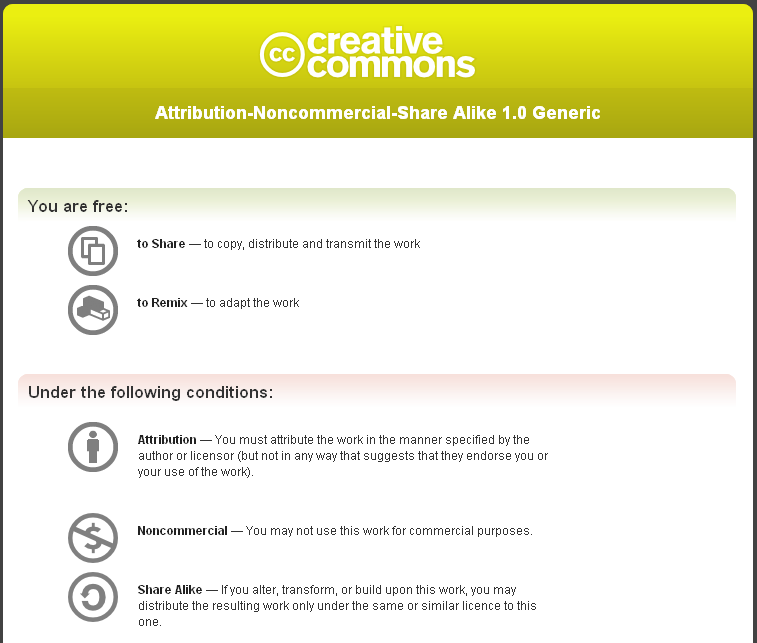
\includegraphics[width=0.65\textwidth]
	{assets/pics/creative_commons.png}
	\caption*{\license}
	\label{fig:lisensi}
\end{figure}

Terkait template ini, gambar lisensi di atas diambil dari \url{http://creativecommons.org/licenses/by-nc-sa/1.0/deed.en_CA}. Jika ingin mengentahui lebih lengkap mengenai \license, silahkan buka \url{http://creativecommons.org/licenses/by-nc-sa/1.0/legalcode}.
Seluruh dokumen yang dibuat dengan menggunakan template ini sepenuhnya menjadi hak milik pembuat dokumen dan bebas didistribusikan sesuai dengan keperluan masing-masing.
Lisensi hanya berlaku jika ada orang yang membuat template baru dengan menggunakan template ini sebagai dasarnya.

Penyusun template ingin berterima kasih kepada Andreas Febrian, Lia Sadita, Fahrurrozi Rahman, Andre Tampubolon, dan Erik Dominikus atas kontribusinya dalam template yang menjadi pendahulu template ini.
Penyusun template juga ingin mengucapkan terima kasih kepada Azhar Kurnia atas kontribusinya dalam template yang menjadi pendahulu template ini.

Semoga template ini dapat membantu orang-orang yang ingin mencoba menggunakan \latex.
Semoga template ini juga tidak berhenti disini dengan ada kontribusi dari para penggunanya.
Jika Anda memiliki perubahan yang dirasa penting untuk disertakan dalam template, silakan lakukan \f{fork} repositori Git template ini di \url{https://gitlab.com/ichlaffterlalu/latex-skripsi-ui-2017}, lalu lakukan \f{merge request} perubahan Anda terhadap \f{branch} \code{master}.
Kami berharap agar \f{template} ini dapat terus diperbarui mengikuti perubahan ketentuan dari pihak Rektorat Universitas Indonesia, dan hal itu tidak mungkin terjadi tanpa kontribusi dari teman-teman sekalian.

% Untuk input gambar tanda tangan, silahkan sesuaikan xshift, yshift, dan width dengan gambar tanda tangan Anda
%\begin{tikzpicture}[remember picture,overlay,shift={(current page.north east)}]
%\node[anchor=north east,xshift=-3cm,yshift=-6.2cm]{
\includegraphics[width=3cm]{assets/pics/tanda_tangan_wikipedia.png}};
%\end{tikzpicture}

\vspace*{0.1cm}
\begin{flushright}
Depok, \tanggalSiapSidang\\[0.1cm]
\ifx\blank\npmDua
	\vspace*{1.5cm}
	\penulisSatu
\else
	Tim Penulis
\fi

\end{flushright}

	\ifodd\thechapterpagecount\forceclearchapter\thispagestyle{onlypage}\fi

	%
	% Lembar Persetujuan Publikasi Ilmiah
	%
	\addChapter{Lembar Persetujuan Karya Ilmiah}
	%
% @author  Andre Tampubolon, Andreas Febrian
% @version 2.2.0
% @edit by Muhammad Aulia Adil Murtito, Ichlasul Affan
%

\chapter*{\uppercase{Halaman Pernyataan Persetujuan Publikasi\\Tugas Akhir untuk Kepentingan Akademis}}
\vspace*{-1cm}
\par\noindent\rule{\textwidth}{3pt}
\vspace*{1cm}
\noindent
Sebagai sivitas akademik Universitas Indonesia,~\ifx\blank\npmDua{saya}\else{kami}\fi~yang bertanda
tangan di bawah ini:

\vspace*{0.2cm}

\pagestyle{onlypage}

\begin{tabular}{p{4.2cm} l p{6.5cm}}
	\ifx\blank\npmDua
	Nama&: & \penulisSatu \\
	NPM&: & \npmSatu \\
	Program Studi&: & \programSatu\\
	\else
	\bo{Penulis 1}\\
	Nama&: & \penulisSatu \\
	NPM&: & \npmSatu \\
	Program Studi&: & \programSatu \vspace*{0.1cm}\\
	\bo{Penulis 2}\\
	Nama&: & \penulisDua \\
	NPM&: & \npmDua \\
	Program Studi&: & \programDua \vspace*{0.1cm}\\
	\fi
	\ifx\blank\npmTiga\else
	\bo{Penulis 3}\\
	Nama&: & \penulisTiga \\
	NPM&: & \npmTiga \\
	Program Studi&: & \programTiga \vspace*{0.1cm}\\
	\fi
	Jenis Karya & : & \type \\
\end{tabular}

\vspace*{0.2cm}

\noindent demi pengembangan ilmu pengetahuan, menyetujui untuk memberikan
kepada Universitas Indonesia \bo{Hak Bebas Royalti Noneksklusif
(\textit{Non-exclusive Royalty Free Right})} atas karya ilmiah~\ifx\blank\npmDua{saya}\else{kami}\fi~yang berjudul:
\begin{center}
	\judul
\end{center}
beserta perangkat yang ada (jika diperlukan). Dengan Hak Bebas Royalti
Noneksklusif ini Universitas Indonesia berhak menyimpan,
mengalihmedia/formatkan, mengelola dalam bentuk pangkalan data
(\textit{database}), merawat, dan memublikasikan tugas akhir~\ifx\blank\npmDua{saya}\else{kami}\fi~selama
tetap mencantumkan nama~\ifx\blank\npmDua{saya}\else{kami}\fi~sebagai penulis/pencipta dan sebagai
pemilik Hak Cipta. \\

\noindent Demikian pernyataan ini~\ifx\blank\npmDua{saya}\else{kami}\fi~buat dengan sebenarnya.

\ifx\blank\npmDua\else\clearpage\fi

% Untuk input gambar tanda tangan, silahkan sesuaikan xshift, yshift, dan width dengan gambar tanda tangan Anda
%\begin{tikzpicture}[remember picture,overlay,shift={(current page.north east)}]
%\node[anchor=north east,xshift=-9cm,yshift=-23.5cm]{
\includegraphics[width=3cm]{assets/pics/tanda_tangan_wikipedia.png}};
%\end{tikzpicture}


\begin{center}
	\vspace*{0.8cm}
	\begin{tabular}{lll}
		Dibuat di&: & Depok \\
		Pada tanggal&: & \tanggalSiapSidang \\
	\end{tabular}\\

	\vspace*{0.2cm}
	Yang menyatakan \\
	\ifx\blank\npmDua
		\vspace*{2cm}
		(\penulisSatu)
	\else
		\begin{multicols}{2}
			Penulis 1:\\
			\vspace*{2cm}
			(\penulisSatu)\\

			Penulis 2:\\
			\vspace*{2cm}
			(\penulisDua)\\
		\end{multicols}
	\fi
	\ifx\blank\npmTiga\else
		\vspace*{0.2cm}
		Penulis 3:\\
		\vspace*{2cm}
		(\penulisTiga)
	\fi
\end{center}

\newpage

	\ifodd\thechapterpagecount\forceclearchapter\thispagestyle{onlypage}\fi
}}


%
% Untuk halaman pertama setiap chapter mulai dari abstrak, tetap berikan mark universitas.
%
\pagestyle{first-pages}


%
% Abstrak
%
\addChapter{Abstrak}
%
% Halaman Abstrak
%
% @author  Andreas Febrian
% @version 2.2.0
% @edit by Ichlasul Affan
%

\chapter*{Abstrak}
\singlespacing

\noindent \begin{tabular}{l l p{10cm}}
	\ifx\blank\npmDua
		Nama&: & \penulisSatu \\
		Program Studi&: & \programSatu \\
	\else
		Nama Penulis 1 / Program Studi&: & \penulisSatu~/ \programSatu\\
		Nama Penulis 2 / Program Studi&: & \penulisDua~/ \programDua\\
	\fi
	\ifx\blank\npmTiga\else
		Nama Penulis 3 / Program Studi&: & \penulisTiga~/ \programTiga\\
	\fi
	Judul&: & \judul \\
	Pembimbing&: & \pembimbingSatu \\
	\ifx\blank\pembimbingDua
    \else
        \ &\ & \pembimbingDua \\
    \fi
    \ifx\blank\pembimbingTiga
    \else
    	\ &\ & \pembimbingTiga \\
    \fi
\end{tabular} \\

\vspace*{0.5cm}

\noindent Isi abstrak. \\

\vspace*{0.2cm}

\noindent Kata kunci: \\ \f{Keyword} satu, kata kunci dua \\

\setstretch{1.4}
\newpage


%
% Halaman Abstract
%
% @author  Andreas Febrian
% @version 2.2.0
% @edit by Ichlasul Affan
%

\chapter*{ABSTRACT}
\singlespacing

\noindent \begin{tabular}{l l p{11.0cm}}
	\ifx\blank\npmDua
		Name&: & \penulisSatu \\
		Study Program&: & \studyProgramSatu \\
	\else
		Writer 1 / Study Program&: & \penulisSatu~/ \studyProgramSatu\\
		Writer 2 / Study Program&: & \penulisDua~/ \studyProgramDua\\
	\fi
	\ifx\blank\npmTiga\else
		Writer 3 / Study Program&: & \penulisTiga~/ \studyProgramTiga\\
	\fi
	Title&: & \judulInggris \\
	Counselor&: & \pembimbingSatu \\
	\ifx\blank\pembimbingDua
	\else
		\ &\ & \pembimbingDua \\
	\fi
	\ifx\blank\pembimbingTiga
	\else
		\ &\ & \pembimbingTiga \\
	\fi
\end{tabular} \\

\vspace*{0.5cm}

\noindent Abstract content. \\

\vspace*{0.2cm}

\noindent Key words: \\ Keyword one, keyword two \\

\setstretch{1.4}
\newpage



%
% Daftar Isi, Gambar, dan Tabel
%

\addDefaultListPage{\tableofcontents}
\addDefaultListPage{\listoffigures}
\addDefaultListPage{\listoftables}


%
% Daftar Kode Program
% Jika tidak digunakan, commment kode ini.
%
\addCustomListPage{\listoflistings}{\lstlistlistingname}


%
% Daftar Equation (Persamaan Matematis)
% Jika bagian ini diperlukan, uncomment kode ini.
%
% \addCustomListPage{\listofequ}{\listofequname}


%
% Daftar Isi yang Didefinisikan Sendiri (Custom)
% Definisi jenis objek baru dapat dilakukan di uithesis.sty
% Jika bagian ini diperlukan, uncomment kode ini.
%
% \addCustomListPage{\listofthing}{\listofthingname}


%
% Daftar Lampiran
% Jika tidak digunakan, commment kode ini.
%
\addCustomListPage{\listofappendix}{\listofappendixname}


% Kembalikan pengaturan chapter dan daftar isi ke aturan awal mulai dari halaman ini
\noCAPinToC
\ifodd\thechapterpagecount\clearpage\else\forceclearchapter\fi

% Jika penomoran romawi selesai di ganjil
% \naiveoddclearchapter
% Jika penomoran romawi selesai di genap
% \naiveevenclearchapter


%
% Gunakan penomoran Arab (1, 2, 3, ...) setelah bagian ini.
%
\pagenumbering{arabic}
\pagestyle{standard}


%
% Isi dari Tugas Akhir/Karya Ilmiah
%
\setoddevenheader
%-----------------------------------------------------------------------------%
\chapter{\babSatu}
\label{bab:1}
%-----------------------------------------------------------------------------%
Pada bab ini, akan dijelaskan tentang latar belakang dan permasalahan yang diselesaikan pada penelitian ini.


%-----------------------------------------------------------------------------%
\section{Latar Belakang}
\label{sec:latarBelakang}
%-----------------------------------------------------------------------------%
\todo{Tentukan latar belakang dari penelitian Anda di sini (\f{background}).}

Tugas Akhir merupakan salah satu kegiatan yang menjadi "penentu nasib" atas lulusnya seorang mahasiswa dari suatu universitas.
Umumnya, mahasiswa yang mengerjakan Tugas Akhir diwajibkan untuk menuliskan sebuah laporan dengan tata bahasa ilmiah dan dengan ketentuan \f{format} tertentu.
Laporan tersebut, memiliki struktur yang kurang lebih mirip, dari manapun fakultas asal seorang mahasiswa.

Umumnya, mahasiswa Universitas Indonesia menggunakan Microsoft Word, OpenOffice, atau \f{rich-text editor} lainnya untuk menyusun laporan Tugas Akhir mereka.
Akan tetapi, terkadang \f{template} yang dibuat untuk Microsoft Word memiliki beberapa keterbatasan dan inkonsistensi dalam pengaturan tata letak.
Selain itu, terdapat beberapa hal yang sulit untuk diotomatisasi, contohnya adalah penggunaan sitasi dan pengaturan nomor halaman.
Oleh karena itu, diperlukan alternatif lain untuk menyusun Tugas Akhir yang lebih nyaman.

Beberapa mahasiswa Fakultas Ilmu Komputer Universitas Indonesia (Fasilkom UI) di tahun 2010-an mulai menggunakan \gls{latex} untuk menyusun Tugas Akhir.
Sifat \gls{latex} yang berupa \f{mark up language}, memiliki cara pemakaian yang jauh berbeda dibandingkan \f{rich-text editor} seperti Microsoft Word.
Awalnya, menyusun tata letak yang sesuai dengan persyaratan Tugas Akhir di UI cukup sulit, karena artinya harus membaca dokumentasi.
Akan tetapi, dengan kemahiran mereka dalam menyusun kode yang mudah dibaca dan terstruktur, struktur yang mereka buat dapat dijadikan sebuah \f{template} yang konsisten tata letaknya hingga bertahun-tahun berikutnya.
Dengan menggunakan sebuah \f{template}, mahasiswa cukup mengetikkan isi dari Tugas Akhir mereka tanpa harus repot mengatur ulang tata letak secara manual.
Mahasiswa bisa menggunakan \f{macro} atau perintab yang sudah disediakan untuk \f{template}.

Adanya perubahan pada peraturan Tugas Akhir yang ditentukan oleh \cite{ui:pedoman_ta}, memunculkan kebutuhan untuk perubahan \f{template} \gls{latex} ini secara signifikan.
Perubahan pada \f{template} ini dilakukan pertama kali pada semester gasal tahun ajaran 2019/2020.
Perubahan dilakukan mengingat adanya kebutuhan dari mahasiswa Lab \f{Reliable Software Engineering} (RSE), Fasilkom UI untuk menyusun Tugas Akhir menggunakan \gls{latex}.
\f{Template} ini kemudian di-\f{maintain} secara berkala, mengikuti umpan balik dan pendapat pengguna \f{template} ini, tidak hanya dari Fasilkom UI, namun juga dari berbagai fakultas lain di UI.
Dengan mulai meluasnya penggunaan \f{template} Tugas Akhir UI ini, diperlukan sebuah contoh penggunaan untuk memudahkan mahasiswa yang baru mulai melaksanakan Tugas Akhir mereka.
Dokumen dan repositori ini, diharapkan selain menjadi repositori kode \f{template}, juga menjadi repositori contoh penggunaan \f{template} dan panduan penggunaan \f{template}.



%-----------------------------------------------------------------------------%
\section{Permasalahan}
\label{sec:masalah}
%-----------------------------------------------------------------------------%
\todo{Sebutkan permasalahan penelitian Anda dari latar belakang tersebut.}

Latar belakang yang telah dijelaskan pada \sect~\ref{sec:latarBelakang}, menjelaskan bahwa diperlukan sebuah \f{template}~\gls{latex} Tugas Akhir UI yang konsisten dan bisa disesuaikan dengan peraturan terbaru dari universitas.
Selain itu, diperlukan juga sebuah \f{tutorial} (panduan penggunaan) yang memudahkan pengguna \f{template} di masa yang akan datang.

%-----------------------------------------------------------------------------%
\subsection{Definisi Permasalahan}
\label{sec:definisiMasalah}
%-----------------------------------------------------------------------------%
Berikut ini adalah rumusan permasalahan dari penelitian yang dilakukan:
\begin{enumerate}
	\item Bagaimana cara menyusun \f{template}~\gls{latex} Tugas Akhir di Universitas Indonesia?
	\item Bagaimana cara mengajarkan penggunaan \f{template} dan bahasa \gls{latex} secara umum ke mahasiswa yang akan menjalani Tugas Akhir?
\end{enumerate}
\todo{Tuliskan permasalahan yang ingin diselesaikan. Bisa juga berbentuk pertanyaan}

%-----------------------------------------------------------------------------%
\subsection{Batasan Permasalahan}
\label{sec:batasanMasalah}
%-----------------------------------------------------------------------------%
Berikut ini adalah asumsi yang digunakan sebagai batasan penelitian ini:
\begin{enumerate}
	\item Salah satu batasannya adalah, ini hanya \f{template}.
\end{enumerate}

\todo{Umumnya ada asumsi atau batasan yang digunakan untuk menjawab pertanyaan-pertanyaan penelitian diatas.}


%-----------------------------------------------------------------------------%
\section{Tujuan Penelitian}
\label{sec:tujuan}
%-----------------------------------------------------------------------------%
Berikut ini adalah tujuan penelitian yang dilakukan:
\begin{enumerate}
	\item Untuk memberikan \f{template} yang dapat mempermudah skripsi orang lain.
\end{enumerate}

\todo{Tuliskan tujuan penelitian Anda di bagian ini.}


%-----------------------------------------------------------------------------%
\section{Manfaat Penelitian}
\label{sec:manfaat}
%-----------------------------------------------------------------------------%
Berikut ini adalah manfaat penelitian yang dilakukan:
\begin{enumerate}
	\item Penelitian ini memberikan \f{template} yang harapannya dapat mempermudah skripsi orang lain.
\end{enumerate}

\todo{Tuliskan tujuan penelitian Anda di bagian ini.}


%-----------------------------------------------------------------------------%
\section{Posisi Penelitian}
\label{sec:posisiPenelitian}
%-----------------------------------------------------------------------------%
\todo{
	Sebutkan posisi penelitian Anda. Ada baiknya jika Anda menggunakan gambar atau diagram.
	Template ini telah menyediakan contoh cara memasukkan gambar.
}

\begin{figure}
	\centering
	
\includegraphics[width=0.4\textwidth]{assets/pics/makara.png}
	\caption{Penjelasan singkat terkait gambar.}
	\label{fig:research_position}
\end{figure}

\todo{
	Jelaskan \pic~\ref{fig:research_position} di sini.
	Setiap gambar yang dimasukkan ke tugas akhir \bo{WAJIB} untuk dijelaskan oleh minimal satu paragraf.
}


%-----------------------------------------------------------------------------%
\section{Langkah Penelitian}
\label{sec:langkahPenelitian}
%-----------------------------------------------------------------------------%
\todo{
	Subbab ini umumnya menjelaskan metode penelitian, jika metode yang digunakan cukup sederhana.
	Jika metode yang digunakan cukup kompleks atau ada kewajiban dari fakultas Anda untuk menjelaskan metode secara rinci, gunakan Bab 3 untuk menjelaskan Metodologi Penelitian.
}
Berikut ini adalah langkah penelitian yang telah dilakukan:
\begin{enumerate}
	\item Tinjauan literatur \\
	Pada tahap ini, dipelajari teori-teori yang terkait dengan penelitian ini untuk mendapatkan konsep dasar yang dibutuhkan dalam mencapai tujuan penelitian.
	\item Analisis implementasi dan kesimpulan \\
	Pada tahap ini, digunakan studi kasus untuk analisis terkait kegunaan \f{template}.
	Setelah melakukan analisis tersebut, ditarik kesimpulan keseluruhan dari penelitian ini.
\end{enumerate}


%-----------------------------------------------------------------------------%
\section{Sistematika Penulisan}
\label{sec:sistematikaPenulisan}
%-----------------------------------------------------------------------------%
Sistematika penulisan laporan adalah sebagai berikut:
\begin{itemize}
	\item Bab 1 \babSatu \\
	    Bab ini mencakup latar belakang, cakupan penelitian, dan pendefinisian masalah.
	\item Bab 2 \babDua \\
	    Bab ini mencakup pemaparan terminologi dan teori yang terkait dengan penelitian berdasarkan hasil tinjauan pustaka yang telah digunakan, sekaligus memperlihatkan kaitan teori dengan penelitian.
	\item Bab 3 \babTiga \\
	    Apa itu Bab 3?
	\item Bab 4 \babEmpat \\
		Apa itu Bab 4?
	\item Bab 5 \babLima \\
	    Apa itu Bab 5?
	\item Bab 6 \kesimpulan \\
	    Bab ini mencakup kesimpulan akhir penelitian dan saran untuk pengembangan berikutnya.
\end{itemize}

\todo{Anda bisa mengubah atau menambahkan penjelasan singkat mengenai isi masing-masing bab. Setiap tugas akhir pasti ada yang berbeda pada bagian ini.}

\clearchapter
%-----------------------------------------------------------------------------%
\chapter{\babDua}
\label{bab:2}
%-----------------------------------------------------------------------------%
\todo{
	Bab ini, biasanya namanya adalah "Studi Literatur" atau "Tinjauan Pustaka".
	Akan tetapi, beberapa fakultas atau dosen pembimbing meminta Bab 2 untuk dinamakan lain, seperti "Kerangka Berpikir".
}

Untuk memulai penelitian, dibutuhkan kerangka berpikir yang sesuai untuk permasalahan yang ingin dipecahkan.
Untuk membentuk kerangka berpikir yang sesuai, perlu dikaitkan dengan hasil studi literatur yang telah dilakukan.
Oleh karena itu, pada bab ini, akan dijelaskan hasil studi literatur yang telah dilakukan yang telah dikaitan dengan kerangka kerja untuk penelitian ini.


%-----------------------------------------------------------------------------%
\section{Apa itu \latex?}
\label{sec:latex}
%-----------------------------------------------------------------------------%

%-----------------------------------------------------------------------------%
\subsection{\latex~Secara Singkat}
\label{sec:latexBrief}
%-----------------------------------------------------------------------------%
Berdasarkan \cite{latex:intro}: \\
\begin{tabular}{| p{14cm} |}
	\hline
	\gls{latex} is a family of programs designed to produce publication-quality typeset documents.
	It is particularly strong when working with mathematical symbols. \\
	The history of \gls{latex} begins with a program called TEX.
	In 1978, a computer scientist by the name of Donald Knuth grew frustrated with the mistakes that his publishers made in typesetting his work.
	He decided to create a typesetting program that everyone could easily use to typeset documents, particularly those that include formulae, and made it freely available.
	The result is TEX. \\
	Knuth's product is an immensely powerful program, but one that does focus very much on small details.
	A mathematician and computer scientist by the name of Leslie Lamport wrote a variant of TEX called \gls{latex} that focuses on document structure rather than such details. \\
	\hline
\end{tabular}

\vspace*{0.2cm}

Dokumen \gls{latex}~sangat mudah, seperti halnya membuat dokumen teks biasa.
Ada beberapa perintah yang diawali dengan tanda '\bslash'.
Seperti perintah \code{\bslash\bslash}~yang digunakan untuk memberi baris baru.
Perintah tersebut juga sama dengan perintah \code{\bslash{}newline}.
Pada bagian ini akan sedikit dijelaskan cara manipulasi teks dan perintah-perintah \gls{latex}~yang mungkin akan sering digunakan.
Jika ingin belajar hal-hal dasar mengenai \gls{latex}, silakan kunjungi:

\begin{itemize}
	\item \url{http://frodo.elon.edu/tutorial/tutorial/}, atau
	\item \url{http://www.maths.tcd.ie/~dwilkins/LaTeXPrimer/}
\end{itemize}

%-----------------------------------------------------------------------------%
\subsection{\latex~Kompiler dan IDE}
\label{sec:latexCompiler}
%-----------------------------------------------------------------------------%
Untuk menggunakan \gls{latex}~(pada konteks hanya sebagai pengguna), tidak perlu banyak tahu mengenai hal-hal didalamnya.
Dengan menggunakan \f{Integrated Development Environment} (IDE), penggunaan \gls{latex}~akan serupa dengan pembuatan dokumen secara visual, layaknya OpenOffice Writer atau Microsoft Word.
Orang-orang yang menggunakan \gls{latex}~relatif lebih teliti dan terstruktur mengenai cara penulisan yang dia gunakan, karena \gls{latex}~memaksa untuk seperti itu.

Untuk mencoba \gls{latex}, diperlukan kompiler dan IDE.
Bagi pengguna Microsoft Windows dan Mac OS, instalasi kompiler \gls{latex}~dapat menggunakan MikTeX (\url{https://miktex.org/download}).
Bagi pengguna Linux, instalasi kompiler \gls{latex}~dapat menggunakan Texlive ( \url{http://www.tug.org/texlive/}).
Distro-distro \f{mainstream} di Linux seperti Ubuntu biasanya telah menyediakan \f{package} \code{texlive} melalui \f{package manager}.
Apabila ingin melakukan instalasi Texlive melalui \f{package manager}, lakukan instalasi package \code{texlive-full} atau setidaknya \code{texlive-science} agar prasyarat \f{template} ini tersedia secara lengkap.

Beberapa text editor atau IDE yang dapat digunakan adalah sebagai berikut:
\begin{itemize}
	\item \underline{\href{https://www.texstudio.org/}{TeXstudio}} (direkomendasikan),
	\item TeXWorks (biasanya bawaan dari \underline{\href{https://miktex.org/download}{MikTeX}}),
	\item \underline{\href{http://www.xm1math.net/texmaker/}{Texmaker}}, atau
	\item Microsoft Visual Studio Code, dengan \f{plugin} \underline{\href{https://marketplace.visualstudio.com/items?itemName=James-Yu.latex-workshop}{\gls{latex} Workshop}}.
	Untuk menggunakan \f{plugin} tersebut, diperlukan instalasi MikTeX dan Perl.
	Alternatif lain untuk persyaratan tersebut adalah menggunakan \f{plugin} Remote - WSL jika memiliki distro Windows Subsystem for Linux (WSL) 2 yang sudah terpasang \code{texlive}.
\end{itemize}


%-----------------------------------------------------------------------------%
\section{\f{Formatting} Teks Dasar}
\label{sec:latexBasicFormatting}
%-----------------------------------------------------------------------------%
Hal pertama yang mungkin ditanyakan adalah bagaimana membuat huruf tercetak tebal, miring, atau memiliki garis bawah.
Pada Texmaker, Anda bisa melakukan hal ini seperti halnya saat mengubah dokumen dengan OO Writer.
Namun jika tetap masih tertarik dengan cara lain, ini dia:

\begin{itemize}
	\item \bo{Bold} \\
	Gunakan perintah \code{\bslash{}textbf$\lbrace\rbrace$} atau
	\code{\bslash{}bo$\lbrace\rbrace$}.\\
	Contoh: \textbf{Contoh hasil tulisan} atau \bo{Contoh hasil tulisan}.
	\item \f{Italic} \\
	Gunakan perintah \code{\bslash{}textit$\lbrace\rbrace$} atau
	\code{\bslash{}f$\lbrace\rbrace$}.\\
	Contoh: \textit{Contoh hasil tulisan} atau \f{Contoh hasil tulisan}.
	\item \underline{Underline} \\
	Gunakan perintah \code{\bslash{}underline$\lbrace\rbrace$}.\\
	Contoh: \underline{Contoh hasil tulisan}.
	\item $\overline{Overline}$ \\
	Gunakan perintah \code{\$\bslash{}overline\$}.\\
	Contoh: $\overline{Contoh~hasil~tulisan}$.
	\item $^{superscript}$ \\
	Gunakan perintah \code{\$\bslash{}$\lbrace\rbrace$\$}.\\
	Contoh: $^{Contoh~hasil~tulisan}$.
	\item $_{subscript}$ \\
	Gunakan perintah \code{\$\bslash{}\_$\lbrace\rbrace$\$}.\\
	Contoh: $_{Contoh~hasil~tulisan}$.
\end{itemize}

% v2.2.1: tutorial dipindah dari Bab 3 ke Bab 2
Ada beberapa hal lain yang bisa digunakan.
\begin{itemize}
	\item Kombinasi \bo{Bold} dan \f{Italic}: \\
	Gunakan perintah \code{\bslash{}bi$\lbrace\rbrace$}. \\
	Contoh: \bi{Contoh hasil tulisan}.
	\item Menebalkan teks formula matematis: \\
	Gunakan perintah \code{\bslash{}m$\lbrace\rbrace$}. \\
	Contoh: \m{\alpha~\beta}
	\item Menebalkan teks formula matematis, sekaligus meletakkannya di tengah: \\
	Gunakan perintah \code{\bslash{}mc$\lbrace\rbrace$}. \\
	Contoh: \mc{\alpha~\beta}
	\item Menggunakan \f{monospaced font} untuk kode:
	Gunakan perintah \code{\bslash{}texttt$\lbrace\rbrace$} atau \code{\bslash{}code$\lbrace\rbrace$}. \\
	Contoh: \texttt{Contoh hasil tulisan} atau \code{Contoh hasil tulisan}.
\end{itemize}

Perintah \code{\bslash{}f}, \code{\bslash{}bo}, \code{\bslash{}bi}, \code{\bslash{}m}, \code{\bslash{}mc},
dan \code{\bslash{}code} hanya dapat digunakan jika package \code{\_internals/uithesis} digunakan.

%-----------------------------------------------------------------------------%
\section{Memasukan Gambar}
\label{sec:latexImage}
%-----------------------------------------------------------------------------%
Setiap gambar dapat diberikan caption dan diberikan label. Label dapat digunakan untuk menunjuk gambar tertentu.
Jika posisi gambar berubah, maka nomor gambar juga akan diubah secara otomatis.
Begitu juga dengan seluruh referensi yang menunjuk pada gambar tersebut.
Contoh sederhana adalah \pic~\ref{fig:testGambar}, yang bisa dibuat dengan menggunakan \lst~\ref{code:latexImage}.
Harap diingat pada aturan Tugas Akhir UI, caption harus selalu \b{diletakkan di bawah gambar}.

\lstinputlisting[language={[latex]tex}, caption=Contoh penggunaan gambar, label=code:latexImage]{assets/codes/tutorial/2-basicFigure.tex}

Berikut adalah penjelasan dari \lst~\ref{code:latexImage}:
\begin{itemize}
	\item Baris ke-2: \code{\bslash{}centering} digunakan untuk membuat gambar berada di tengah.
	\item Baris ke-3 dan 4: \code{\bslash{}includegraphics} digunakan untuk memasukkan gambar. \\
	\code{width=0.25\bslash{}textwidth} digunakan untuk mengatur lebar gambar sebesar 25\% dari lebar teks (dari ujung marjin kiri ke ujung marjin kanan).
	\item Baris ke-5: \code{\bslash{}caption} digunakan untuk memberikan \f{caption} pada gambar.
	\f{Caption} tersebut diletakkan setelah \code{includegraphics} agar \f{caption} berada di bawah gambar.
	\item Baris ke-6: \code{\bslash{}label} digunakan untuk memberikan label pada gambar.
	Label ini bisa digunakan di suatu paragraf untuk merujuk pada gambar tersebut,
	dengan cara menuliskan \code{\bslash{}ref\{label\}} pada paragraf.
\end{itemize}

\begin{figure}
	\centering
	
\includegraphics[width=0.25\textwidth]
	{assets/pics/makara_kuning.png}
	\caption{Makara Universitas Indonesia}
	\label{fig:testGambar}
\end{figure}


Anda juga bisa memasukkan sitasi atau URL sumber gambar, jika gambar tersebut bukan Anda sendiri yang membuatnya.
Contoh sederhana adalah \pic~\ref{fig:testGambarBersumber}, yang bisa dibuat dengan menggunakan \lst~\ref{code:latexImageSource}.

\lstinputlisting[language={[latex]tex}, caption=Contoh penggunaan gambar bersumber, label=code:latexImageSource]{assets/codes/tutorial/2-sourcedFigure.tex}

Pada baris ke-5, \code{\bslash{}captionsource} digunakan untuk memberikan caption dan sumber gambar.
Dalam kasus ini, sumber gambar merupakan sebuah URL, sehingga ditandai dengan perintah \code{\bslash{}url\{\}}.
Jika sumber gambar merupakan sebuah buku, jurnal, atau dokumen, maka bisa dilakukan sitasi menggunakan perintah \code{\bslash{}cite\{\}}.
Contoh: \code{\bslash{}captionsource\{Sesuatu\}\{\bslash{}cite\{latex:intro\}\}}.

\begin{figure}
	\centering
	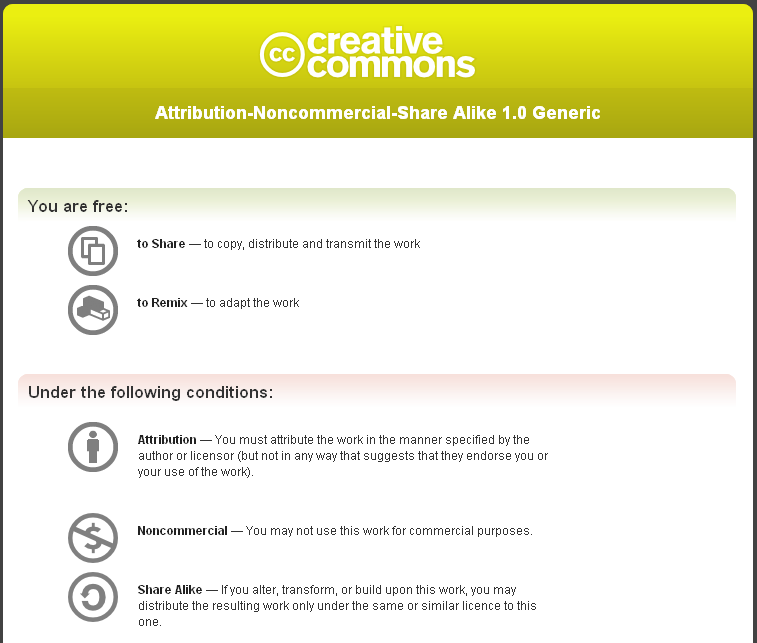
\includegraphics[width=0.50\textwidth]
	{assets/pics/creative_commons.png}
	\captionsource{\license.}{{\url{https://creativecommons.org/licenses/by-nc-sa/1.0/}}}
	\label{fig:testGambarBersumber}
\end{figure}



%-----------------------------------------------------------------------------%
\section{Membuat Tabel}
\label{sec:latexTable}
%-----------------------------------------------------------------------------%
Tabel pada \gls{latex} dapat dibuat secara visual dengan bantuan \f{website} seperti \url{https://www.tablesgenerator.com/}.
Dengan menggunakan \textit{website} ini, maka pembuatan tabel akan menjadi lebih mudah.
\textit{User interface} dari \f{website} dapat dilihat pada Gambar \ref{fig:tablesgenerator}.

\begin{figure}
	\centering
	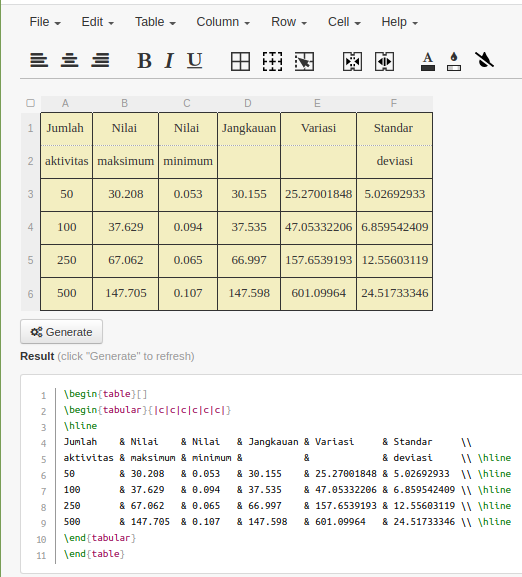
\includegraphics[width=0.5\textwidth]{assets/pics/tablesgenerator-dot-com.png}
	\caption{\textit{User interface} dari \textit{website} https://www.tablesgenerator.com/}
	\label{fig:tablesgenerator}
\end{figure}

Di sisi lain, tabel juga dapat diberi label dan caption seperti pada gambar.
Caption pada tabel terletak pada bagian atas tabel.
Contoh kode yang menyusun suatu tabel sederhana dapat dilihat pada \lst~\ref{code:latexTable}.

\lstinputlisting[language={[latex]tex}, caption=Contoh penggunaan tabel, label=code:latexTable]{assets/codes/tutorial/2-basicTable.tex}

Berikut adalah penjelasan dari \lst~\ref{code:latexTable}:
\begin{itemize}
	\item Baris ke-2: \code{\bslash{}centering} digunakan untuk membuat tabel berada di tengah.
	\item Baris ke-3: \code{\bslash{}caption} digunakan untuk memberikan \f{caption} pada tabel.
	\f{Caption} tersebut diletakkan setelah \code{begin\{tabular\}} agar \f{caption} berada di atas tabel.
	\item Pada baris ke-3, terdapat argumen \code{| l | c r |} yang artinya adalah sebagai berikut:
	\begin{itemize}
		\item \code{|} digunakan untuk membuat garis vertikal pada tabel.
		\item \code{l} digunakan untuk membuat suatu kolom menjadi rata kiri.
		\item \code{c} digunakan untuk membuat suatu kolom menjadi rata tengah.
		\item \code{r} digunakan untuk membuat suatu kolom menjadi rata kanan.
	\end{itemize}
	\item Baris ke-4: \code{\bslash{}label} digunakan untuk memberikan label pada tabel.
	Label ini bisa digunakan di suatu paragraf untuk merujuk pada tabel tersebut,
	dengan cara menuliskan \code{\bslash{}ref\{label\}} pada paragraf.
	\item Baris ke-5: \code{\bslash{}begin\{tabular\}} digunakan untuk memulai pembuatan tabel.
	\item \code{\bslash{}hline} digunakan untuk membuat garis horizontal pada tabel.
	\item \code{\&} digunakan untuk memisahkan antar kolom.
	\item \code{\bslash{}\bslash{}} digunakan untuk memisahkan antar baris.
	\item Baris ke-17 dan 18: Kode untuk mengakhiri pembuatan tabel.
\end{itemize}

Hasil dari \lst~\ref{code:latexTable} akan menjadi \tab~\ref{tab:basic}.

\begin{table}
	\centering
	\caption{Contoh Tabel}
	\label{tab:basic}
	\begin{tabular}{| l | c r |} %
		\hline % garis lurus horizontal
		& kol 1 & kol 2 \\ % baris 1
		\hline %
		baris 1 & 1 & 2 \\ % baris 2
		baris 2 & 3 & 4 \\ % baris 3
		baris 3 & 5 & 6 \\ % baris 4
		baris 4 & 7 & 8 \\ % baris 5
		baris 5 & 9 & 10 \\ % baris 6
		\hline
		\bo{jumlah} & \bo{25} & \bo{30} \\ % baris 7
		\hline
	\end{tabular}
\end{table}



%-----------------------------------------------------------------------------%
\subsection{Tabel Panjang (Lintas Baris)}
\label{sec:latexLongTable}
%-----------------------------------------------------------------------------%
Adapun untuk membuat tabel panjang yang bisa melebihi dari satu halaman,
gunakan perintah \code{\bslash{}begin\{longtable\}} sebagai pengganti \code{\bslash{}begin\{table\}}.
Di dalam \code{longtable} tidak perlu lagi ada \code{\bslash{}begin\{tabular\}}.
Kemudian, tambahkan tanda \code{\bslash{}\bslash{}} setelah baris \code{\bslash{}label\{....\}},
agar tidak menimbulkan error saat menampilkan \f{caption} di bagian atas tabel.
Kemudian, untuk membatasi header yang ingin diulang pada halaman-halaman berikutnya,
gunakan perintah \code{\bslash{}endhead}.
Contoh kode pembuatan tabel pankang dapat dilihat pada \lst~\ref{code:latexLongTable}.

\lstinputlisting[language={[latex]tex}, caption=Contoh penggunaan tabel panjang, label=code:latexLongTable]{assets/codes/tutorial/2-longTable.tex}

Terdapat lima bagian pada sebuah tabel panjang:
\begin{enumerate}
	\item Awalan (\f{header}) di halaman pertama, umumnya disebut sebgai \code{firsthead}.\\
	Pada \lst~\ref{code:latexLongTable}, bagian ini didefinisikan di baris 2 sampai 7.
	Bagian ini diakhiri definisinya dengan perintah \code{\bslash{}endfirsthead}.
	Pada bagian ini, \f{caption} yang digunakan merupakan \f{caption} asli.
	\code{caption} dan \code{label} hanya perlu didefinisikan di bagian awal tabel, di halaman pertama saja.
	Anda juga tetap bisa menggunakan \code{captionsource} apabila dibutuhkan.
	\item Awalan (\f{header}) di halaman berikutnya, umumnya disebut sebagai \code{head}.\\
	Pada \lst~\ref{code:latexLongTable}, bagian ini didefinisikan di baris 8 sampai 12.
	Bagian ini diakhiri definisinya dengan perintah \code{\bslash{}endhead}.
	Terkait penggunaan \f{caption} sambungan:
	\begin{itemize}
		\item Jika Anda menggunakan \code{\bslash{}caption\{\}}, maka untuk menuliskan caption sambungan, gunakan perintah \code{\bslash{}caption[]\{\}}.
		Pada kasus \lst~\ref{code:latexLongTable}, \f{caption} sambungan didefinisikan di baris 8 menggunakan perintah \code{\bslash{}caption[]\{\}}.
		\item Jika Anda menggunakan \code{\bslash{}captionsource\{\}\{\}}, maka untuk menuliskan caption sambungan, gunakan perintah \code{\bslash{}captionsourcecont\{\}\{\}}.
	\end{itemize}
	\item Akhiran (\f{footer}) yang muncul di halaman pertama hingga sebelum terakhir, umumnya disebut sebagai \code{foot}.\\
	Bagian ini diakhiri definisinya dengan perintah \code{\bslash{}endfoot}.
	Pada \lst~\ref{code:latexLongTable}, bagian ini didefinisikan di baris 13 sampai 14.
	Dalam kasus ini, akhiran tabel hanya berupa garis horizontal.
	\item Akhiran (\f{footer}) di halaman terakhir, umumnya disebut sebagai \code{lastfoot}.\\
	Bagian ini diakhiri definisinya dengan perintah \code{\bslash{}endlastfoot}.
	Pada \lst~\ref{code:latexLongTable}, bagian ini didefinisikan di baris 15 sampai 16.
	Dalam kasus ini, akhiran tabel hanya berupa garis horizontal.
	\item Isi dari tabel.
	Pada \lst~\ref{code:latexLongTable}, bagian ini didefinisikan di baris 17 sampai 32.
	Isi dari tabel akan diletakkan di antara awalan tabel (\f{header}) dan akhiran tabel (\f{footer}).
\end{enumerate}

Hasil dari \lst~\ref{code:latexLongTable} akan menjadi \tab~\ref{tab:long}.

\begin{longtable}{| l | c r |}
    \caption{Contoh Tabel Panjang}
    \label{tab:long} \\
    \hline
    & kol 1 & kol 2 \\
    \hline
    \endfirsthead % batas akhir header yang akan muncul di halaman pertama
    \caption[]{Contoh Tabel Panjang (sambungan)} \\
    \hline
    & kol 1 & kol 2 \\
    \hline
    \endhead % batas akhir header yang akan muncul di halaman berikutnya
    \hline
    \endfoot % batas akhir footer yang akan muncul di halaman berikutnya
    \hline
    \endlastfoot % batas akhir footer yang akan muncul di halaman terakhir
    baris 1  & 1 & 2 \\
    baris 2  & 3 & 4 \\
    baris 3  & 5 & 6 \\
    baris 4  & 7 & 8 \\
    baris 5  & 9 & 10 \\
    baris 6  & 11 & 12 \\
    baris 7  & 13 & 14 \\
    baris 8  & 15 & 16 \\
    baris 9  & 17 & 18 \\
    baris 10 & 19 & 20 \\
    baris 11 & 21 & 22 \\
    baris 12 & 23 & 24 \\
    baris 13 & 25 & 26 \\
    baris 14 & 27 & 28 \\
    baris 15 & 29 & 30 \\
    baris 16 & 31 & 32 \\
\end{longtable}


%-----------------------------------------------------------------------------%
\subsection{Menggabungkan (\f{Merge}) Baris atau Kolom}
\label{sec:latexMergeCellsTable}
%-----------------------------------------------------------------------------%
Ada jenis tabel lain yang dapat dibuat dengan \gls{latex}~berikut beberapa diantaranya.
Contoh-contoh ini bersumber dari \url{https://en.wikibooks.org/wiki/LaTeX/Tables}.

\bo{Contoh 1: Menggabungkan Kolom} \\
Contoh penggunaan tabel dengan sel yang melebar ke lebih dari satu kolom dapat dilihat pada \lst~\ref{code:mergeColumnTable}.
Pada contoh ini, sel pada baris 1, kolom 3 dan 4 digabungkan menjadi satu dengan menggunakan perintah \code{\bslash{}multicolumn\{3\}\{c\}\{Week 1\}}.

\lstinputlisting[language={[latex]tex}, caption=Contoh penggunaan tabel dengan sel yang melebar ke lebih dari satu kolom, label=code:mergeColumnTable]{assets/codes/tutorial/2-mergeColumnTable.tex}

Hasil dari \lst~\ref{code:mergeColumnTable} akan menjadi \tab~\ref{tab:rowSpanning}.

\begin{table}
	\centering
	\captionsource{Tabel dengan sel yang melebar ke lebih dari satu kolom}{\url{https://en.wikibooks.org/wiki/LaTeX/Tables}, dengan modifikasi.}
	\label{tab:rowSpanning}
	\begin{tabular}{|l|l|*{6}{c|}}
		% Baris 1
		\hline % buat garis horizontal dari kolom pertama ke kolom terakhir
		No & Name & \multicolumn{3}{|c|}{Week 1} & \multicolumn{3}{|c|}{Week 2} \\
		% Baris 2
		\cline{3-8} % buat garis horizontal dari kolom 3 sampai 8
		& & A & B & C & A & B & C\\
		% Baris 3
		\hline
		1 & Lala & 1 & 2 & 3 & 4 & 5 & 6\\
		% Baris 4
		2 & Lili & 1 & 2 & 3 & 4 & 5 & 6\\
		% Baris 5
		3 & Lulu & 1 & 2 & 3 & 4 & 5 & 6\\
		\hline
	\end{tabular}
\end{table}


\bo{Contoh 2: Menggabungkan Baris} \\
Contoh penggunaan tabel dengan sel yang melebar ke lebih dari satu baris dapat dilihat pada \lst~\ref{code:mergeRowTable}.
Pada contoh ini, sel pada kolom 1, baris 2 dan 3 digabungkan menjadi satu dengan menggunakan perintah \code{\bslash{}multirow\{2\}\{*\}\{Kedua\}}.

\lstinputlisting[language={[latex]tex}, caption=Contoh penggunaan tabel dengan sel yang melebar ke lebih dari satu baris, label=code:mergeRowTable]{assets/codes/tutorial/2-mergeRowTable.tex}

Hasil dari \lst~\ref{code:mergeRowTable} akan menjadi \tab~\ref{tab:columnSpanning}.

\begin{table}
	\centering
	\captionsource{Tabel dengan sel yang melebar ke lebih dari satu baris}{\url{https://en.wikibooks.org/wiki/LaTeX/Tables}, dengan modifikasi.}
	\label{tab:columnSpanning}
	\begin{tabular}{|l|c|l|} % border vertikal ditandai dengan |
        % Baris 1
		\hline % buat garis horizontal dari kolom pertama ke kolom terakhir
		Percobaan & Iterasi & Waktu \\
        % Baris 2
		\hline
		Pertama & 1 & 0.1 sec \\ \hline
        % Baris 3 (kolom 1 melebar 2 baris)
		\multirow{2}{*}{Kedua} & 1 & 0.1 sec \\
        % Baris 4 (kolom 1 dikosongkan karena sudah ditimpa)
		& 3 & 0.15 sec \\
        % Baris 5 (kolom 1 melebar 3 baris)
		\hline
		\multirow{3}{*}{Ketiga} & 1 & 0.09 sec \\
        % Baris 6 (kolom 1 dikosongkan karena sudah ditimpa)
		& 2 & 0.16 sec \\
        % Baris 7 (kolom 1 dikosongkan karena sudah ditimpa)
		& 3 & 0.21 sec \\
		\hline
	\end{tabular}
\end{table}


\bo{Contoh 3: Menggabungkan Baris dan Kolom} \\
Contoh penggunaan tabel dengan sel yang melebar ke lebih dari satu kolom dan baris dapat dilihat pada \lst~\ref{code:mergeBothTable}.

\lstinputlisting[language={[latex]tex}, caption=Contoh penggunaan tabel dengan sel yang melebar ke lebih dari satu kolom dan baris, label=code:mergeBothTable]{assets/codes/tutorial/2-mergeBothTable.tex}

Hasil dari \lst~\ref{code:mergeBothTable} akan menjadi \tab~\ref{tab:mixSpanning}.

\begin{table}
	\centering
	\captionsource{Tabel dengan sel yang melebar ke lebih dari satu kolom dan baris}{\url{https://en.wikibooks.org/wiki/LaTeX/Tables}, dengan modifikasi.}
	\label{tab:mixSpanning}
	\begin{tabular}{|cc|c|c|c|c|} % border vertikal ditandai dengan |, semua kolom rata tengah.
        % 2-row 2-col span (rata tengah), dan 4-col span (rata tengah)
		\hline % buat garis horizontal dari kolom pertama ke kolom terakhir
		\multicolumn{2}{|c|}{\multirow{2}{*}{Element}} & \multicolumn{4}{c|}{Title} \\
        % kelanjutan border untuk 2-row 2-col span, dan 4 kolom biasa
        \cline{3-6} % buat garis horizontal dari kolom 3 sampai 6
		\multicolumn{2}{|c|}{} & A & B & C & D \\
        % 2-row span (rata kiri), dan 5 kolom biasa
        \hline
		\multicolumn{1}{|l|}{\multirow{2}{*}{Type}} & X & 1 & 2 & 3 & 4 \\
        % kelanjutan border untuk 2-row span, dan 5 kolom biasa
        \cline{2-6}
		\multicolumn{1}{|l|}{} & Y & 0.5 & 1.0 & 1.5 & 2.0 \\
        % kelanjutan bordering untuk 2-row span, dan 5 kolom biasa
        % 2-row span (rata kiri), dan 5 kolom biasa
        \hline
		\multicolumn{1}{|l|}{\multirow{2}{*}{Resource}} & I & 10 & 20 & 30 & 40\\
        % kelanjutan border untuk 2-row span, dan 5 kolom biasa
        \cline{2-6}
		\multicolumn{1}{|l|}{} & J & 5 & 10 & 15 & 20 \\
        \hline
	\end{tabular}
\end{table}




%-----------------------------------------------------------------------------%
\section{Membuat Persamaan Matematis}
\label{sec:mathEqu}
%-----------------------------------------------------------------------------%
% v2.2.1: tutorial dipindah dari Bab 3 ke Bab 2
Di \gls{latex}, kita dapat membuat persamaan matematis baik yang terdiri dari satu persamaan maupun lebih dari satu persamaan.
Anda bisa mencoba mengikuti dan memahami contoh kode yang ada di \f{template} ini untuk kebutuhan tugas akhir Anda.
Menggunakan \gls{latex}~juga perlu latihan dan lihai memahami dokumentasi.

%-----------------------------------------------------------------------------%
\subsection{Satu Persamaan}
\label{sec:oneEqu}
%-----------------------------------------------------------------------------%
\noindent \begin{align}\label{equ:garis}
	\cfrac{y - y_{1}}{y_{2} - y_{1}} =
	\cfrac{x - x_{1}}{x_{2} - x_{1}}
\end{align}

\addequtotoc{equ:garis}{Persamaan garis}


\equ~\ref{equ:garis} di atas adalah persamaan garis.
Persamaan tersebut dapat disusun dengan menggunakan perintah \code{\bslash{}align}, seperti yang ditunjukkan pada \lst~\ref{code:singleEquationGaris}.
Penggunaan perintah \code{\bslash{}noindent} sebelum memanggil \f{environment} \code{align} diperlukan agar persamaan yang dicetak tidak tergeser mengikuti indentasi yang umumnya muncul di awal paragraf.
Terdapat beberapa perintah yang digunakan untuk menyusun \equ~\ref{equ:garis}, yaitu:
\begin{itemize}
	\item Perintah \code{\bslash{}cfrac\{\}\{\}} untuk menulis pecahan dalam bentuk vertikal.
	Argumen pertama adalah pembilang (di atas), sedangkan argumen kedua adalah penyebut (di bawah).
	\item Perintah \code{\bslash{}\_\{\}} untuk menulis \f{subscript}.
\end{itemize}

Di luar \f{environment} \code{align}, kita juga bisa menambahkan persamaan tersebut ke daftar persamaan dengan menggunakan perintah \code{\bslash{}addequtotoc\{label\}\{caption\}}.
Perintah \code{\bslash{}label} pada persamaan matematis hanya akan memberikan label,
namun tidak menambahkan ke daftar persamaan.
Perintah \code{\bslash{}addequtotoc} harus ditambahkan di luar \f{environment} \code{align},
karena perintah tersebut harus dijalankan di mode \f{typesetting} teks biasa agar tidak terjadi \f{error}.

\lstinputlisting[language={[latex]tex}, caption=Kode pembuatan \equ~\ref{equ:garis}, label=code:singleEquationGaris]{assets/codes/tutorial/2-singleEquationGaris.tex}

Persamaan bola berikut, yang ditunjukkan oleh \ref{equ:bola}, merupakan contoh lain menyusun sebuah persamaan di \gls{latex}.

\noindent \begin{align}\label{equ:bola}
	\underbrace{|\overline{ab}|}_{\text{pada bola $|\overline{ab}| = r$}}
	= \sqrt[2]{(x_{b} - x_{a})^{2} + (y_{b} - y_{a})^{2} +
		\vert\vert(z_{b} - z_{a})^{2}}
\end{align}

\addequtotoc{equ:bola}{Persamaan bola}


Terdapat beberapa perintah yang digunakan untuk menyusun \equ~\ref{equ:bola}, yaitu:
\begin{itemize}
	\item Perintah \code{\bslash{}sqrt\{\}} untuk menulis akar.
	\item Perintah \code{\bslash{}underbrace\{\}} untuk menulis \f{brace} di bawah suatu ekspresi.
		Biasanya digunakan untuk memberikan anotasi terhadap suatu ekspresi.
	\item Perintah \code{\bslash{}overline\{\}} untuk menulis garis di atas suatu ekspresi.
	\item Perintah \code{\bslash{}text\{\}} untuk menulis teks biasa di dalam persamaan.
	\item Di dalam teks biasa, kita bisa menuliskan kembali sebuah persamaan matematis dengan menambahkan tanda \code{\$} di awal dan di akhir persamaan tersebut.
		Di \gls{latex}, terdapat dua mode \f{typesetting}, yaitu mode teks dan mode matematika.
		Fungsi \code{\$} adalah untuk mengubah mode teks menjadi mode matematika.
	\item Perintah \code{\bslash{}vert} untuk menulis tanda garis vertikal.
\end{itemize}

\lstinputlisting[language={[latex]tex}, caption=Kode pembuatan \equ~\ref{equ:bola}, label=code:singleEquationBola]{assets/codes/tutorial/2-singleEquationBola.tex}

Suatu persamaan yang dibuat menggunakan \f{environment} \code{align} akan secara otomatis memiliki indeks (nomor) dari persamaan.
Perintah \code{align} ini juga dapat digunakan untuk menulis lebih dari satu persamaan.


%-----------------------------------------------------------------------------%
\subsection{Lebih dari Satu Persamaan}
\label{sec:multiEqu}
%-----------------------------------------------------------------------------%
\equ~\ref{equ:matriks} adalah contoh persamaan matriks yang dibuat menggunakan \gls{latex}.

\noindent \begin{align}\label{equ:matriks}
	|\overline{a} * \overline{b}| &= |\overline{a}| |\overline{b}| \sin\theta
	\\[0.2cm]
	\overline{a} * \overline{b} &=
	\begin{array}{| c c c |}
		\hat{i} & x_{1} & x_{2} \\
		\hat{j} & y_{1} & y_{2} \\
		\hat{k} & z_{1} & z_{2} \\
	\end{array} \nonumber \\[0.2cm]
	&= \hat{i} \,
	\begin{array}{ | c c | }
		y_{1} & y_{2} \\
		z_{1} & z_{2} \\
	\end{array}
	+ \hat{j} \,
	\begin{array}{ | c c | }
		z_{1} & z_{2} \\
		x_{1} & x_{2} \\
	\end{array}
	+ \hat{k} \,
	\begin{array}{ | c c | }
		x_{1} & x_{2} \\
		y_{1} & y_{2} \\
	\end{array}
	\nonumber
\end{align}

\addequtotoc{equ:matriks}{Persamaan matriks}


Pada \equ~\ref{equ:matriks} dapat dilihat beberapa baris persamaan menjadi satu bagian dari persamaan tersebut.
Kode untuk menyusun kumpulan persamaan di \equ~\ref{equ:matriks} dapat dilihat pada \lst~\ref{code:multiEquationAsOne}.
Eksekusi perintah \code{\bslash{}addequtotoc\{label\}\{caption\}} juga cukup dilakukan sekali saja.

\lstinputlisting[language={[latex]tex}, caption=Kode pembuatan \equ~\ref{equ:matriks}, label=code:multiEquationAsOne]{assets/codes/tutorial/2-multiEquationAsOne.tex}

Terdapat beberapa perintah yang digunakan untuk menyusun \equ~\ref{equ:matriks}, yaitu:
\begin{itemize}
	\item Perintah \code{\bslash{}begin\{array\}} dan \code{\bslash{}end\{array\}} untuk membuat matriks.
	Cara kerja \f{environment} \code{array} sama dengan \f{environment} \code{tabular} yang digunakan untuk membuat tabel.
	\item Perintah \code{\bslash{}sin} untuk menulis fungsi sinus.
	\item Perintah \code{\bslash{}theta} untuk menulis simbol theta ($\theta$).
	\item Perintah \code{\bslash{}hat\{\}} untuk menulis tanda aksen \f{hat} (\^{}) di atas suatu huruf.
\end{itemize}

Sedangkan dibawah ini dapat dilihat bahwa dengan cara yang sama, \equ~
\ref{equ:integral}, \ref{equ:limit}, dan \ref{equ:eksponen} memiliki nomor
persamaannya masing-masing.

\noindent \begin{align}
	\label{equ:integral}
	\int_{a}^{b} f(x)\, dx + \int_{b}^{c} f(x) \, dx = \int_{a}^{c} f(x) \, dx \\
	\label{equ:limit}
	\lim_{x \to \infty} \frac{f(x)}{g(x)} = 0 \hspace{1cm}
	\text{jika pangkat $f(x)$ $<$ pangkat $g(x)$} \\
	\label{equ:eksponen}
	a^{m^{a \, ^{n}\log b }} = b^{\frac{m}{n}}
\end{align}

\addequtotoc{equ:integral}{Persamaan integral}
\addequtotoc{equ:limit}{Persamaan limit}
\addequtotoc{equ:eksponen}{Persamaan eksponen dan logaritma}


Kode yang menyusun \equ~\ref{equ:integral}, \ref{equ:limit}, dan \ref{equ:eksponen} dapat dilihat pada \lst~\ref{code:multiEquationAsSeparate}.
Perbedaan penyusunan tiga argumen tersebut dibandingkan dengan \equ~\ref{equ:matriks} adalah penggunaan \f{label} pada setiap persamaan.
Pada \equ~\ref{equ:matriks}, \f{label} diletakkan pada bagian awal persamaan pertama, sehingga hanya satu \f{label} yang digunakan.
Pada \equ~\ref{equ:integral}, \ref{equ:limit}, dan \ref{equ:eksponen}, \f{label} diletakkan pada awal setiap persamaan, sehingga setiap persamaan memiliki \f{label} masing-masing.
Selain itu, jika ingin memasukkan setiap persamaan secara terpisah ke Daftar Persamaan,
eksekusi perintah \code{\bslash{}addequtotoc\{label\}\{caption\}} juga harus dilakukan terpisah untuk setiap persamaan.

\lstinputlisting[language={[latex]tex}, caption={Kode pembuatan \equ~\ref{equ:integral}, \ref{equ:limit}, dan \ref{equ:eksponen}}, label=code:multiEquationAsSeparate]{assets/codes/tutorial/2-multiEquationAsSeparate.tex}

Terdapat beberapa perintah yang digunakan untuk menyusun \equ~\ref{equ:integral}, \ref{equ:limit}, dan \ref{equ:eksponen}, yaitu:
\begin{itemize}
	\item Perintah \code{\bslash{}int} untuk menulis simbol integral.
	Untuk batas bawah dan batas atas integral, bisa dituliskan dengan menggunakan perintah \f{subscript} dan \f{superscript}.
	\item Perintah \code{\bslash{}lim} untuk menulis simbol limit.
	\item Perintah \code{\bslash{}to} untuk menulis panah ke kanan.
	\item Perintah \code{\bslash{}infty} untuk menulis simbol tak hingga.
	\item Perintah \code{\bslash{}log} untuk menulis fungsi logaritma.
	Pangkat basis logaritma dituliskan dengan menggunakan perintah \f{superscript} sebelum perintah \code{\bslash{}log}.
\end{itemize}


%-----------------------------------------------------------------------------%
\section{Menambahkan Kode Program}
\label{sec:codeListing}
% Hal baru di template 2017
%-----------------------------------------------------------------------------%
% v2.2.1: tutorial dipindah dari Bab 3 ke Bab 2
Pada \gls{latex}, kode program seringkali disebut \f{listing}.
\f{Syntax highlighting} kini sudah bisa dilakukan secara otomatis oleh \f{library} yang ada di \gls{latex}.
Sudah tidak perlu lagi membuat skrip manual untuk menambahkan \f{syntax highlighting} sendiri.
\lst~\ref{code:java} adalah contoh kode program (\f{listing}) Java yang dicetak oleh \gls{latex}.

\lstinputlisting[language=Java, caption=Kode sampel Java yang cukup panjang, label=code:java]{assets/codes/2-sample.java}

Sintaks untuk memasukkan kode program ke dalam dokumen \gls{latex}~adalah sebagai berikut:

\begin{lstlisting}[language={[latex]tex}, caption=Meng]
\lstinputlisting[language=Java, caption=Kode sampel Java yang cukup panjang, label=code:java]{assets/codes/2-sample.java}
\end{lstlisting}

Terdapat tiga argumen yang digunakan pada perintah \code{\bslash{}lstinputlisting}:
\begin{itemize}
	\item \code{language} digunakan untuk menentukan bahasa pemrograman yang digunakan.
	Untuk menggunakan suatu dialek bahasa pemrograman yang berbeda dari \f{default},
	misalkan versi Python3 dari Python,
	gunakan perintah \code{language=\{[3]Python\}}.
	\item \code{caption} digunakan untuk memberikan \f{caption} pada kode program.
	Argumen ini sifatnya opsional, jika ada, maka \f{caption} akan ditampilkan di bawah kode program.
	Jika argumen ini tidak ada, maka \f{caption} tidak akan ditampilkan dan kode tidak bisa masuk ke daftar kode program.
	\item \code{label} digunakan untuk memberikan label pada kode program untuk rujukan di dalam dokumen (\f{cross-reference}).
	Argumen ini tidak boleh didefinisikan jika argumen \code{caption} tidak didefinisikan.
\end{itemize}

Terdapat empat kelompok bahasa pemrograman (dan dialek) yang didukung oleh implementasi \code{listings} pada \f{template} ini, yaitu:

\begin{itemize}
	\item \bo{Bahasa pemrograman yang didukung secara \f{default} oleh \code{listings}} (menurut \cite{latex:source_code_listings}): \\
		\code{ABAP}, \code{ACSL}, \code{Ada}, \code{Algol}, \code{Ant}, \code{Awk}, \code{bash}, \code{Basic}, \code{C++}, \code{C}, \code{Caml},
		\code{Clean}, \code{Cobol}, \code{Comal}, \code{command.com} (Windows Batch), \code{csh}, \code{Delphi}, \code{Eiffel}, \code{Elan},
		\code{erlang}, \code{Euphoria}, \code{Fortran}, \code{GCL}, \code{Go} (golang), \code{Gnuplot}, \code{Haskell}, \code{HTML}, \code{IDL},
		\code{inform}, \code{Java}, \code{JVMIS}, \code{ksh}, \code{Lisp}, \code{Logo}, \code{Lua}, \code{make}, \code{Mathematica}, \code{Matlab},
		\code{Mercury}, \code{MetaPost}, \code{Miranda}, \code{Mizar}, \code{ML}, \code{Modelica}, \code{Modula-2}, \code{MuPAD}, \code{NASTRAN},
		\code{Oberon-2}, \code{OCL}, \code{Octave}, \code{Oz}, \code{Pascal}, \code{Perl}, \code{PHP}, \code{PL/I}, \code{Plasm}, \code{POV},
		\code{Prolog}, \code{Promela}, \code{PSTricks}, \code{Python}, \code{R}, \code{Reduce}, \code{Rexx}, \code{RSL}, \code{Ruby}, \code{S},
		\code{SAS}, \code{Scilab}, \code{sh}, \code{SHELXL}, \code{Simula}, \code{SQL}, \code{tcl}, \code{TeX}, \code{VBScript}, \code{Verilog},
		\code{VHDL}, \code{VRML}, \code{XML}, dan \code{XSLT}.
	\item \bo{Dialek yang didukung secara \f{default} oleh \code{listings}} (menurut \cite{latex:source_code_listings}, diambil beberapa contoh):
		\begin{itemize}
			\item Dialek Assembly: \code{[Motorola68k]\{Assembler\}}, \code{[x86masm]\{Assembler\}},
			\item Dialek Awk: \code{[gnu]\{Awk\}} (GNU Awk), \code{[POSIX]\{Awk\}},
			\item Dialek C: \code{[ANSI]\{C\}} (default), \code{[Handel]\{C\}}, \code{[Objective]\{C\}} (Objective-C), \code{[Sharp]\{C\}} (C\#),
			\item Dialek Caml: \code{[Objective]\{Caml\}} (OCaml), \code{[light]\{Caml\}} (default),
			\item Dialek C++: \code{[11]\{C++\}}, \code{[ANSI]\{C++\}}, \code{[GNU]\{C++\}}, \code{[Visual]\{C++\}} (Visual C++),
				\code{[ISO]\{C++\}} (default),
			\item Dialek Java: \code{[]\{Java\}} (default), \code{[AspectJ]\{Java\}},
			\item Dialek Pascal: \code{[Borland6]\{Pascal\}}, \code{[XSC]\{Pascal\}}, \code{[Standard]\{Pascal\}} (default),
			\item Dialek Python: \code{[2]\{Python\}} (default, Python 2), \code{[3]\{Python\}} (Python 3),
			\item Dialek TeX: \code{[LaTeX]\{TeX\}} (LaTeX), \code{[AlLaTeX]\{TeX\}}, \code{[plain]\{TeX\}} (plain TeX, default),
			\item Dialek tcl: \code{[]\{Tcl\}} (default Tcl), \code{[tk]\{Tcl\}} (Tcl/Tk).
		\end{itemize}
	\item \bo{Bahasa pemrograman yang ditambahkan pada \f{template} ini}: \\
		\code{ABS}, \code{Acceleo}, \code{Batch}, \code{Clojure}, \code{CSS}, \code{D}, \code{Dart}, \code{Docker}, \code{F\#} (FSharp),
		\code{GDScript} (Godot), \code{GLSL}, \code{Groovy}, \code{HLSL}, \code{JavaScript}, \code{Julia}, \code{Kotlin}, \code{Markdown},
		\code{PowerShell}, \code{Rust}, \code{Scala}, \code{Scheme}, \code{Solidity}, \code{Swift}, \code{TOML}, \code{TypeScript}, dan \code{YAML}.
	\item \bo{Dialek yang ditambahkan pada \f{template} ini}:
		\begin{itemize}
			\item Dialek HTML: \code{[v5]\{HTML\}} (HTML5),
			\item Dialek Java: \code{[v9]\{Java\}} (Java 9 Modules), \code{[ContextJ]\{Java\}}, \code{[DeltaJ]\{Java\}}, dan \code{[FOP]\{Java\}}.
		\end{itemize}
\end{itemize}

Berikut adalah contoh penggunaan dialek bahasa pemrograman dalam menuliskan kode program.
Dalam kasus ini, \lst~\ref{code:python2} merupakan kode Python versi 2.
Sedangkan, \lst~\ref{code:python3} merupakan kode Python versi 3.
Perbedaan antara kedua versi tersebut cukup signifikan, salah satunya adalah pada perintah \code{print}.
Pada Python 2, perintah \code{print} tidak memerlukan tanda kurung karena merupakan sebuah \f{keyword},
sedangkan pada Python 3, perintah \code{print} memerlukan tanda kurung karena merupakan sebuah \f{function}.

\lstinputlisting[language=Python, caption=Kode Python 2, label=code:python2]{assets/codes/2-sample-python2.py}

\lstinputlisting[language={[3]Python}, caption=Kode Python 3, label=code:python3]{assets/codes/2-sample-python3.py}

Kode yang mencetak \lst~\ref{code:python2} dan \lst~\ref{code:python3} adalah sebagai berikut:

\begin{lstlisting}[language={[latex]tex}]
\lstinputlisting[language=Python, caption=Kode Python 2, label=code:python2]{assets/codes/2-sample-python2.py}
\lstinputlisting[language={[3]Python}, caption=Kode Python 3, label=code:python3]{assets/codes/2-sample-python3.py}
\end{lstlisting}

Secara \f{default}, dialek yang digunakan untuk Python pada \f{library} \code{listings} adalah Python 2.
Sehingga untuk mencetak kode Python 3, perlu digunakan dialek Python 3 (\code{\{[3]Python\}}).

Kode program yang dicetak oleh \gls{latex} bersifat \f{auto-wrapped}.
Jika suatu baris kode program melebihi batas lebar halaman,
maka kode program tersebut akan dipindahkan ke baris berikutnya.
\f{Auto-wrapped} ini berguna agar Anda tidak perlu memberikan \f{line break} manual pada kode Anda,
Anda bisa menyampaikan kode program Anda apa adanya.

\bo{Catatan}: Jangan lupa untuk menjelaskan kode melalui paragraf,
terutama pada bagian-bagian yang perlu penjelasan lebih.
Setiap kode perlu dijelaskan, kalau bisa rujuk ke setiap baris, karena belum tentu pembaca mau membaca kode Anda.
Tetapi, pembaca tetap perlu mengetahui ide di balik kode yang Anda buat, dan mengapa kode tersebut dibuat.



%-----------------------------------------------------------------------------%
\section{Keterkaitan Teori Dengan Penelitian}
\label{sec:keterkaitan}
%-----------------------------------------------------------------------------%
\todo{
	Ada baiknya setelah menjelaskan teori-teori, Anda menjelaskan apa kaitan teori tersebut dengan penelitian Anda.
	Hal ini tentunya membantu pembaca dalam memahami bahwa teori yang Anda paparkan memang penting untuk memahami penelitian Anda nantinya.
}

\begin{figure}
	\centering
	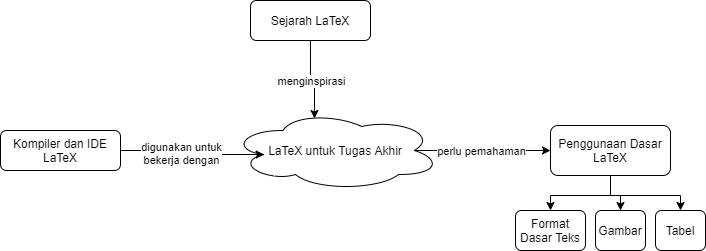
\includegraphics[width=\textwidth]{assets/pics/research_concept_map.png}
	\caption{Keterkaitan konsep hasil studi literatur terhadap penelitian}
	\label{fig:research_concept_map}
\end{figure}

\todo{
	Jelaskan \pic~\ref{fig:research_concept_map} di sini.
	Setiap gambar pada tugas akhir butuh penjelasan.
	Gambar hadir untuk mempermudah membaca memahami konteks, tetapi tidak bisa berdiri sendiri tanpa penjelasan.
}

\clearchapter
%-----------------------------------------------------------------------------%
\chapter{\babTiga}
\label{bab:3}
%-----------------------------------------------------------------------------%
Bab ini menjelaskan tentang hal-hal \f{advanced} dalam \gls{latex}.
Hal ini mencakup bagaimana cara menulis persamaan matematis di \gls{latex}, menambahkan daftar isi, catatan, \acrshort{pdf}, menambahkan kode, bahkan menambahkan perintah baru.

\todo{
	Sejatinya bab ini digunakan untuk membahas inti dari penelitian Anda.
	Sesuaikan saja dengan kebutuhkan Anda: misalkan bab tiga Anda adalah penjelasan terkait desain sistem.
}


%-----------------------------------------------------------------------------%
\section{Melakukan \f{Cross-Reference} ke Suatu Bagian dalam Laporan}
\label{sec:crossReference}
%-----------------------------------------------------------------------------%
Dengan menggunakan \gls{latex}, Anda tidak perlu lagi melakukan referensi ke suatu bagian atau objek dalam laporan secara manual.
Anda cukup melakukan referensi ke bagian/gambar/kode/persamaan yang Anda inginkan dengan menggunakan perintah \code{\bslash{}ref}.
Anda tidak perlu lagi mengubah referensi secara manual setiap kali ada perubahan letak pada bagian tersebut, karena \gls{latex}~akan melakukannya secara otomatis.
Selain itu, pada berkas \acrfull{pdf} yang dihasilkan oleh \gls{latex}, referensi tersebut akan memiliki \f{link} yang langsung mengarahkan pembaca ke posisi objek atau bagian yang direferensikan.
Untuk melakukan \f{cross-reference}, pertama kali tandai bagian yang ingin Anda referensikan dengan menggunakan suatu label, melalui perintah \code{\bslash{}label\{...:.....\}}.
Label tidak boleh mengandung spasi. Berikut ini adalah konvensi penamaan label dan cara melakukan referensi yang digunakan dalam \f{template} ini:
\begin{itemize}
	\item \code{\bslash{}label\{bab:[nomorBab]\}} untuk sebuah bab. \\
	Contoh: \code{\bslash{}label\{bab:3\}} \\
	Cara referensi: \code{\bslash{}bab\~\bslash{}ref\{bab:3\}} \\
	Hasil referensi: \bab~\ref{bab:3}.
	\item \code{\bslash{}label\{sec:[....]\}} untuk sebuah subbab. \\
	Contoh: \code{\bslash{}label\{sec:crossReference\}} \\
	Cara referensi: \code{\bslash{}sect\~\bslash{}ref\{sec:crossReference\}} \\
	Hasil referensi: \sect~\ref{sec:crossReference}.
	\item \code{\bslash{}label\{appendix:[....]\}} untuk sebuah bab/subbab lampiran. \\
	Contoh: \code{\bslash{}label\{appendix:changelog\}} \\
	Cara referensi: \code{\bslash{}apdx\~\bslash{}ref\{appendix:changelog\}} \\	Hasil referensi: \apdx~\ref{appendix:changelog}.
	\item \code{\bslash{}label\{equ:[....]\}} untuk sebuah persamaan matematis. \\
	Contoh: \code{\bslash{}label\{equ:matriks\}} \\
	Cara referensi: \code{\bslash{}equ\~\bslash{}ref\{equ:matriks\}} \\
	Hasil referensi: \equ~\ref{equ:matriks}.
	\item \code{\bslash{}label\{fig:[....]\}} untuk sebuah gambar. \\
	Contoh: \code{\bslash{}label\{fig:testGambar\}} \\
	Cara referensi: \code{\bslash{}pic\~\bslash{}ref\{fig:testGambar\}} \\
	Hasil referensi: \pic~\ref{fig:testGambar}.
	\item \code{\bslash{}label\{tab:[....]\}} untuk sebuah tabel. \\
	Contoh: \code{\bslash{}label\{tab:\tab1\}} \\
	Cara referensi: \code{\bslash{}tab\~\bslash{}ref\{tab:tab1\}} \\
	Hasil referensi: \tab~\ref{tab:long}.
	\item Untuk sebuah kode sumber, label diletakkan sebagai argumen dari \code{\bslash{}lstinputlisting} seperti: \code{\bslash{}lstinputlisting[..., label=code:...]}. \\
	Contoh: \code{\bslash{}lstinputlisting[language=Java, caption=Kode sampel Java, label=code:java]} \\
	Cara referensi: \code{\bslash{}lst\~\bslash{}ref\{code:java\}} \\
	Hasil referensi: \lst~\ref{code:java}.
\end{itemize}


%-----------------------------------------------------------------------------%
\section{Menggunakan BibTeX}
\label{sec:bibtex}
% Hal baru di template 2017
%-----------------------------------------------------------------------------%
BibTeX adalah \f{library} dalam \gls{latex}~yang dapat membantu Anda untuk menuliskan sitasi.
Dengan menggunakan BibTeX, Anda tidak perlu memikirkan format penulisan referensi atau sitasi.
\f{Formatting} akan dilakukan secara otomatis sesuai dengan format sitasi yang digunakan.
Secara \f{default}, \f{template} ini menggunakan format sitasi APA.
Namun, format tersebut dapat diubah sesuai dengan peraturan yang dimiliki oleh fakultas, dosen pembimbing, atau dosen penguji Anda.

%-----------------------------------------------------------------------------%
\subsection{Menambahkan Referensi}
\label{sec:bibtexAddRef}
%-----------------------------------------------------------------------------%
Anda bisa menambahkan bahan bacaan yang ingin Anda jadikan referensi ke dalam berkas \code{references.bib}.
Contoh isi kode \f{references.bib} saat ini dapat dilihat di \lst~\ref{code:references}.
\lstinputlisting[language=TeX, caption=Daftar referensi di \code{references.bib}, label=code:references, linerange={1-12}]{config/references.bib}

Format suatu objek referensi pada BibTex adalah sebagai berikut: \\
\code{@[tipe-referensi]\{[kode-untuk-sitasi]}\\
\code{\indent\hspace{5ex}title~~~~=~\{Judul Buku\},}\\
\code{\indent\hspace{5ex}....}\\
\code{\}}\\
Kode untuk sitasi dapat berisi karakter non-spasi yang bisa digunakan untuk melakukan sitasi di dalam konten laporan.
Terdapat empat belas tipe referensi yang bisa digunakan pada BibTeX:
\begin{itemize}
	\item \code{article}: Digunakan untuk merujuk ke sebuah artikel dalam suatu majalah, buku, atau koleksi artikel lainnya.
	\item \code{book}: Digunakan untuk merujuk ke sebuah buku.
	\item \code{booklet}: Digunakan untuk merujuk ke sebuah buku saku.
	\item \code{inbook}: Digunakan untuk merujuk ke sebuah bab atau subbab dalam suatu buku.
	\item \code{incollection}: Digunakan untuk merujuk ke sebuah bab atau subbab dalam suatu koleksi atau seri buku.
	\item \code{mastersthesis}: Digunakan untuk merujuk ke sebuah tesis karya mahasiswa magister (S2).
	\item \code{manual}: Digunakan untuk merujuk ke suatu buku manual.
	\item \code{phdthesis}: Digunakan untuk merujuk ke sebuah tesis karya mahasiswa doktoral (S3).
	\item \code{proceedings}: Digunakan untuk merujuk ke sebuah \f{paper} ilmiah yang dipublikasikan dalam suatu \f{conference} atau prosiding.
	\item \code{techreport}: Digunakan untuk merujuk ke suatu laporan teknis (misal: draf konvensi teknologi terbaru).
	\item \code{unpublished}: Digunakan untuk merujuk ke suatu hal yang tidak dipublikasikan.
	\item \code{misc}: Digunakan untuk merujuk ke hal-hal lain yang tidak masuk ke kategori-kategori yang telah disebutkan.
\end{itemize}

%-----------------------------------------------------------------------------%
\subsection{Melakukan Sitasi pada Konten Tugas Akhir}
\label{sec:bibtexAddCite}
%-----------------------------------------------------------------------------%
Berikut ini adalah contoh kalimat yang menggunakan sitasi: \\
"Kalimat menurut \cite{book:sample} terdiri dari subjek, predikat, dan objek \citep{book:sample}."

Berikut adalah kode yang digunakan untuk melakukan sitasi pada kalimat tersebut:
\begin{lstlisting}[language={[latex]tex}]
	"Kalimat menurut \cite{book:sample} terdiri dari subjek, predikat, dan objek \citep{book:sample}."
\end{lstlisting}

Ada format sitasi yang memiliki cara penulisan yang berbeda berdasarkan posisi sitasi, ada juga yang tidak.
Format sitasi APA membedakan penulisan sitasi pada isi kalimat dengan akhir kalimat, sedangkan format sitasi IEEE tidak.
\f{Template} ini menggunakan format sitasi APA secara \f{default}, sehingga diperlukan pembeda berdasarkan posisi sitasi.
Untuk melakukan sitasi pada isi kalimat, di mana sitasi tersebut umumnya sebagai subjek, objek, atau keterangan pada kalimat, gunakan perintah \code{\bslash{}citep}.
Sedangkan untuk melakukan sitasi pada akhir kalimat, di mana sitasi tersebut umumnya sebagai rujukan suatu gagasan, gunakan perintah \code{\bslash{}cite}.

Perlu diperhatikan bahwa \code{\bslash{}citep} hanya bisa digunakan untuk format sitasi yang butuh membedakan posisi sitasi.
Penggunaan \code{\bslash{}citep} pada format sitasi seperti IEEE akan menimbulkan error.
Jika Anda menggunakan format seperti itu, cukup gunakan \code{\bslash{}cite} dimanapun posisi sitasi Anda.

%-----------------------------------------------------------------------------%
\subsection{Mengubah Format Referensi/Sitasi}
\label{sec:bibtexChangeFormat}
% Hal baru di template 2017
%-----------------------------------------------------------------------------%
Sejak versi \f{template} 2.0.2, format referensi \f{default} telah diganti menjadi APA dari sebelumnya IEEE karena banyaknya permintaan dosen penguji untuk menggunakan format APA.
Pada dasarnya, peraturan Rektor UI terkait Tugas Akhir menyerahkan format referensi sesuai dengan aturan fakultas.
Namun, mayoritas dari fakultas atau dosen pembimbing di Universitas Indonesia menggunakan APA sebagai format sitasinya.
Oleh karena itu, jika fakultas atau dosen pembimbing/penguji Anda meminta format sitasi yang berbeda selain APA, Anda bisa menggantinya dengan mengikuti tahapan berikut:
\begin{enumerate}
	\item Pada berkas \code{uithesis.sty}, terdapat bagian \bo{Package}. Cari konfigurasi "Format sitasi".
	\item Hilangkan tanda komentar (\f{uncomment}) pada bagian konfigurasi format yang akan digunakan, misal: APA. Pastikan hanya satu jenis konfigurasi format yang di-\f{uncomment}.
	\item Cari "Konfigurasi khusus sitasi APA" di bagian \bo{Ubah Istilah Penulisan}.
	\begin{itemize}
		\item Jika Anda akan menggunakan format APA, hilangkan tanda komentar (\f{uncomment}) pada bagian konfigurasi tersebut.
		\item Jika Anda akan menggunakan format selain APA, jadikan bagian konfigurasi tersebut sebagai komentar (\f{comment}).
	\end{itemize}
	\item Tidak semua format sitasi mengenal perbedaan pada sitasi di awal/tengah kalimat atau di akhir kalimat.
	Contoh format yang mengenal perbedaan tersebut adalah APA dan MLA.
	IEEE dan ACM tidak mengenal format tersebut.
	\begin{itemize}
		\item Jika format sitasi yang akan digunakan mengenal perbedaan tersebut, ganti sitasi pada akhir kalimat atau tempat lain yang membutuhkan model sitasi dengan \f{parentheses} (kurung) dengan menggunakan perintah \code{\bslash{}citep}.
		\item Jika format sitasi yang akan digunakan tidak mengenal perbedaan tersebut, pastikan semua sitasi menggunakan perintah \code{\bslash{}cite}.
	\end{itemize}
	\item Jika muncul pesan error seperti \code{[nama-format].bst not found}, itu tandanya format tersebut tidak tersedia secara bawaan dari BibTeX.
	Unduh berkas terkait dahulu dari CTAN, lalu letakkan di direktori \code{\_internals}.
	Contoh format sitasi yang membutuhkan berkas eksternal adalah MLA (konfigurasi MLA sudah tersedia di \code{uithesis.sty}, namun berkas \code{mla.bst} belum tersedia).
	\item Jika konfigurasi format sitasi belum tersedia di \code{uithesis.sty}, ikuti langkah-langkah berikut:
	\begin{enumerate}
		\item Tambahkan konfigurasi baru di \code{uithesis.sty}, pada bagian \bo{Package} $>$ "Format sitasi".
		Contoh bisa mengikuti dengan format-format lain yang sudah tersedia, namun silakan sesuaikan dengan kebutuhan format sitasi yang akan digunakan.
		\item Jika format sitasi yang akan digunakan mengenal perbedaan pada sitasi di awal/tengah kalimat atau di akhir kalimat, gunakan \f{package} \code{natbib} sehingga mendukung \f{command} sitasi \code{\bslash{}citep}.
	\end{enumerate}
\end{enumerate}


%-----------------------------------------------------------------------------%
\section{Membuat Daftar Istilah (Glosarium)}
\label{sec:glossary}
% Hal baru di template 2017
%-----------------------------------------------------------------------------%
Daftar istilah atau glosarium adalah daftar kata atau frasa yang digunakan dalam dokumen beserta definisinya.
Daftar frasa tersebut bisa berupa istilah, atau berupa singkatan/akronim.
Template ini sudah menggunakan \f{library} \code{glossaries}.
Berikut adalah langkah-langkah untuk mendefinisikan istilah baru atau singkatan/akronim baru dan menggunakannya dalam dokumen Anda.

\subsection{Menambahkan Istilah atau Akronim Baru}
Untuk menambahkan istilah atau akronim baru, buka berkas \code{config/istilah.tex}
dan tambahkan definisi istilah atau akronim baru menggunakan perintah \code{\bslash{}newglossaryentry} atau \code{\bslash{}newacronym}.

\begin{lstlisting}[language={[latex]tex}, caption=Contoh definisi istilah baru, label=code:newTerm]
\newglossaryentry{latex}{
	name={\LaTeX},
	description={A document preparation system for high-quality typesetting}
}
\end{lstlisting}

Pada \lst~\ref{code:newTerm}, ditunjukkan bahwa \code{\bslash{}newglossaryentry} memiliki 3 argumen, yaitu:
\begin{itemize}
	\item Argumen \f{positional} pertama: Merupakan kode panggilan untuk istilah tersebut.
		Kode tersebut yang nanti akan digunakan untuk memanggil istilah tersebut dalam dokumen.
	\item Argumen \f{keyword} \code{name}: Merupakan istilah yang akan dicetak ke dalam dokumen jika definisi ini dipanggil.
		Contoh: Jika \code{\bslash{}gls\{latex\}} dipanggil, maka yang akan dicetak adalah \gls{latex}.
	\item Argumen \f{keyword} \code{description}: Definisi (deskripsi) dari istilah tersebut.
		Deskripsi tersebut nantinya akan muncul di halaman Daftar Istilah.
\end{itemize}

\begin{lstlisting}[language={[latex]tex}, caption=Contoh definisi singkatan/akronim baru, label=code:newAcronym]
\newacronym{pdf}{PDF}{Portable Document Format}
\end{lstlisting}

Pada \lst~\ref{code:newAcronym}, ditunjukkan bahwa \code{\bslash{}newacronym} memiliki 3 argumen, yaitu:
\begin{itemize}
	\item Argumen pertama: Merupakan kode panggilan untuk akronim tersebut.
	\item Argumen kedua:
		Merupakan akronim (dalam bentuk singkatan) yang akan dicetak ke dalam dokumen jika definisi ini dipanggil menggunakan \code{\bslash{}acrshort}.
		Contoh: Jika \code{\bslash{}acrshort\{pdf\}} dipanggil, maka yang akan dicetak adalah \acrshort{pdf}.
	\item Argumen ketiga:
		Kepanjangan dari akronim tersebut.
		Kepanjangan ini akan dicetak ke dalam dokumen jika definisi ini dipanggil menggunakan \code{\bslash{}acrlong} atau \code{\bslash{}acrfull}.
		Contoh:
		\begin{itemize}
			\item \code{\bslash{}acrlong\{pdf\}} akan mencetak \acrlong{pdf}.
			\item \code{\bslash{}acrfull\{pdf\}} akan mencetak \acrfull{pdf}.
		\end{itemize}
\end{itemize}

\subsection{Menggunakan Istilah atau Akronim dalam Dokumen}
Setelah mendefinisikan istilah atau akronim, Anda dapat menggunakannya dalam dokumen dengan perintah \code{\bslash{}gls}, \code{\bslash{}glspl}, \code{\bslash{}acrshort}, \code{\bslash{}acrlong}, atau \code{\bslash{}acrfull}. Contoh:

\begin{lstlisting}[language={[latex]tex}, caption=Contoh penggunaan istilah atau akronim dalam dokumen, label=code:useTerm]
\gls{latex} adalah sistem persiapan dokumen untuk pengetikan berkualitas tinggi.
\acrfull{pdf} adalah format berkas yang digunakan untuk representasi dokumen dua dimensi.
\acrlong{pdf} merupakan format berkas yang dibuat oleh Adobe.
\acrshort{pdf} dapat di-\f{edit} menggunakan Adobe Acrobat.
\end{lstlisting}

\lst~\ref{code:useTerm} akan menghasilkan kalimat berikut:

\begin{tabular}{| p{\linewidth} |}
	\hline
	\gls{latex} adalah sistem persiapan dokumen untuk pengetikan berkualitas tinggi.
	\acrfull{pdf} adalah format berkas yang digunakan untuk representasi dokumen dua dimensi.
	\acrlong{pdf} merupakan format berkas yang dibuat oleh Adobe.
	\acrshort{pdf} dapat di-\f{edit} menggunakan Adobe Acrobat. \\
	\hline
\end{tabular}
\vspace{0.2cm}


%-----------------------------------------------------------------------------%
\section{Memasukan Berkas PDF}
\label{sec:pdf}
%-----------------------------------------------------------------------------%
Untuk memasukan berkas \acrfull{pdf} dapat menggunakan perintah \code{\bslash{}inpdf} yang menerima satu buah argumen.
Argumen ini berisi nama berkas yang akan digabungkan dalam laporan.
\acrshort{pdf} yang dimasukan dengan cara ini akan memiliki header dan footer seperti pada halaman lainnya.

\inpdf{assets/pdfs/include}

Cara lain untuk memasukan \acrshort{pdf} adalah dengan menggunakan perintah \code{\bslash{}putpdf} dengan satu argumen yang berisi nama berkas pdf.
Berbeda dengan perintah sebelumnya, \acrshort{pdf} yang dimasukan dengan cara ini tidak akan memiliki footer atau header seperti pada halaman lainnya.

\putpdf{assets/pdfs/include}


%-----------------------------------------------------------------------------%
\section{Memberikan Catatan}
\label{sec:note}
%-----------------------------------------------------------------------------%
Ada dua perintah untuk memberikan catatan penulisan dalam dokumen yang Anda kerjakan, yaitu:
\begin{itemize}
	\item \code{\bslash{}todo} \\
	Contoh: \\
	\noindent\hspace{-1em}\todo{Contoh bentuk todo.}
	\item \code{\bslash{}todoCite} \\
	Contoh: \todoCite
\end{itemize}


%-----------------------------------------------------------------------------%
\section{\f{Layoutting} Tingkat Lanjut}
\label{sec:advancedLayoutting}
% Hal baru di template 2017
%-----------------------------------------------------------------------------%

%-----------------------------------------------------------------------------%
\subsection{Menambahkan Tabel/Gambar Panjang secara Lanskap}
\label{sec:landscape}
% Hal baru di template 2017
%-----------------------------------------------------------------------------%
Ketika Anda ingin memasukkan tabel atau gambar yang ukurannya cukup panjang ke samping, Anda diperkenankan untuk menyajikan konten tersebut dengan orientasi \f{landscape}.
Caranya cukup mudah, yaitu dengan menambahkan \code{\bslash{}begin\{landscape\}} di sebelum konten dan \code{\bslash{}end\{landscape\}} di setelah konten.
Format ini kompatibel juga dengan \code{longtable} untuk tabel yang panjang dan lebar. Contoh penggunaannya adalah pada \tab~\ref{tab:longTableLandscape}.

\begin{landscape}
\begin{footnotesize}
\begin{longtable}{ | l | l | l | l | l | l | l | l | l | l | l | l | l | l | }
	\captionsource{Contoh Tabel: Data Kasus COVID-19 di Asia, 14 September 2020}{\url{https://worldometers.info/coronavirus}}
	\label{tab:longTableLandscape} \\
	\hline
	\multirow{2}{*}{\#} & \multirow{2}{*}{Country, Other} & \multicolumn{2}{|c|}{Cases} & \multicolumn{2}{|c|}{Deaths} & \multicolumn{2}{|c|}{Recovered} & \multirow{2}{*}{Active} & \multirow{2}{*}{Critical} & \multicolumn{3}{|c|}{.../1M pop} & \multirow{2}{*}{Population} \\
	& & Total & New & Total & New & Total & New & & & Tot Cases & Deaths & Tests & \\ \hline
	\endfirsthead % batas akhir header yang akan muncul di halaman pertama
	\captionsourcecont{Contoh Tabel: Data Kasus COVID-19 di Asia, 14 September 2020}{\url{https://worldometers.info/coronavirus}} \\
	\hline
	\multirow{2}{*}{\#} & \multirow{2}{*}{Country, Other} & \multicolumn{2}{|c|}{Cases} & \multicolumn{2}{|c|}{Deaths} & \multicolumn{2}{|c|}{Recovered} & \multirow{2}{*}{Active} & \multirow{2}{*}{Critical} & \multicolumn{3}{|c|}{.../1M pop} & \multirow{2}{*}{Population} \\
	& & Total & New & Total & New & Total & New & & & Tot Cases & Deaths & Tests & \\ \hline
	\endhead % batas akhir header yang akan muncul di halaman berikutnya
	1 & India & 4850887 & 5884 & 79784 & 30 & 3780107 & 3063 & 990996 & 8944 & 3508 & 58 & 41395 & 1382752528 \\ \hline
	2 & Iran & 404648 & 2619 & 23313 & 156 & 348013 & 1771 & 33322 & 3798 & 4805 & 277 & 42594 & 84209239 \\ \hline
	3 & Bangladesh & 339332 & 1812 & 4759 & 26 & 243155 & 2512 & 91418 &  & 2056 & 29 & 10560 & 165021623 \\ \hline
	4 & Saudi Arabia & 325651 &  & 4268 &  & 302870 &  & 18513 & 1326 & 9325 & 122 & 163863 & 34922248 \\ \hline
	5 & Pakistan & 302020 & 539 & 6383 & 4 & 289806 & 377 & 5831 & 551 & 1362 & 29 & 13388 & 221741906 \\ \hline
	6 & Turkey & 291162 &  & 7056 &  & 258833 &  & 25273 & 1267 & 3445 & 83 & 100796 & 84522503 \\ \hline
	7 & Iraq & 290309 &  & 8014 &  & 224705 &  & 57590 & 546 & 7186 & 198 & 46610 & 40399964 \\ \hline
	8 & Philippines & 265888 & 4699 & 4630 & 259 & 207504 & 249 & 53754 & 1048 & 2420 & 42 & 28018 & 109874163 \\ \hline
	9 & Indonesia & 221523 & 3141 & 8841 & 118 & 158405 & 3395 & 54277 &  & 808 & 32 & 9751 & 274108479 \\ \hline
	10 & Israel & 156823 & 1219 & 1126 & 7 & 115128 & 130 & 40569 & 529 & 17050 & 122 & 297533 & 9197590 \\ \hline
	11 & Qatar & 121740 &  & 205 &  & 118682 &  & 2853 & 37 & 43358 & 73 & 246111 & 2807805 \\ \hline
	12 & Kazakhstan & 106855 & 52 & 1634 &  & 100627 & 12 & 4594 & 221 & 5677 & 87 & 136625 & 18821980 \\ \hline
	13 & Kuwait & 94764 &  & 560 &  & 84995 &  & 9209 & 94 & 22124 & 131 & 157765 & 4283219 \\ \hline
	14 & Oman & 90222 & 476 & 790 & 10 & 83928 & 157 & 5504 & 171 & 17580 & 154 & 60252 & 5131974 \\ \hline
	15 & China & 85194 & 10 & 4634 &  & 80415 & 16 & 145 & 2 & 59 & 3 & 111163 & 1439323776 \\ \hline
	16 & UAE & 79489 &  & 399 &  & 69451 &  & 9639 &  & 8017 & 40 & 819752 & 9914483 \\ \hline
	17 & Japan & 75218 &  & 1439 &  & 66899 &  & 6880 & 180 & 595 & 11 & 13576 & 126395837 \\ \hline
	18 & Bahrain & 60307 &  & 212 &  & 53681 &  & 6414 & 29 & 35209 & 124 & 731472 & 1712845 \\ \hline
	19 & Singapore & 57454 & 48 & 27 &  & 56764 &  & 663 &  & 9805 & 5 & 389287 & 5859703 \\ \hline
	20 & Nepal & 54159 &  & 345 &  & 38697 &  & 15117 &  & 1852 & 12 & 28745 & 29240966 \\ \hline
	21 & Uzbekistan & 47620 & 333 & 394 & 4 & 44002 & 136 & 3224 & 246 & 1419 & 12 & 41050 & 33566409 \\ \hline
	22 & Armenia & 45969 & 107 & 919 & 3 & 41693 & 34 & 3357 &  & 15507 & 310 & 81279 & 2964385 \\ \hline
	23 & Kyrgyzstan & 44928 & 47 & 1063 &  & 41023 & 101 & 2842 & 24 & 6864 & 162 & 40900 & 6545664 \\ \hline
	24 & Afghanistan & 38772 & 56 & 1425 & 5 & 32073 & 435 & 5274 & 93 & 992 & 36 & 2741 & 39100693 \\ \hline
	25 & Azerbaijan & 38327 &  & 562 &  & 35756 &  & 2009 &  & 3773 & 55 & 98716 & 10157722 \\ \hline
	26 & Palestine & 30574 &  & 221 &  & 20082 &  & 10271 &  & 5966 & 43 & 66248 & 5124685 \\ \hline
	27 & Lebanon & 24310 &  & 241 &  & 8334 &  & 15735 & 113 & 3565 & 35 & 94995 & 6819062 \\ \hline
	28 & S. Korea & 22285 & 109 & 363 & 5 & 18489 & 263 & 3433 & 157 & 435 & 7 & 41948 & 51278298 \\ \hline
	29 & Malaysia & 9946 & 31 & 128 &  & 9203 & 7 & 615 & 11 & 307 & 4 & 42286 & 32449426 \\ \hline
	30 & Maldives & 9173 &  & 32 &  & 7326 &  & 1815 & 12 & 16911 & 59 & 240315 & 542438 \\ \hline
	31 & Tajikistan & 9049 &  & 72 &  & 7816 &  & 1161 &  & 945 & 8 &  & 9579764 \\ \hline
	32 & Syria & 3540 &  & 155 &  & 842 &  & 2543 &  & 201 & 9 &  & 17583867 \\ \hline
	33 & Thailand & 3475 & 2 & 58 &  & 3312 &  & 105 & 1 & 50 & 0.8 & 10728 & 69836028 \\ \hline
	34 & Jordan & 3314 &  & 24 &  & 2206 &  & 1084 & 13 & 324 & 2 & 95814 & 10223646 \\ \hline
	35 & Sri Lanka & 3234 &  & 12 &  & 3005 & 9 & 217 &  & 151 & 0.6 & 11844 & 21431662 \\ \hline
	36 & Myanmar & 3015 & 83 & 24 & 4 & 699 &  & 2292 &  & 55 & 0.4 & 3518 & 54484197 \\ \hline
	37 & Georgia & 2392 & 165 & 19 &  & 1369 &  & 1004 &  & 600 & 5 & 118041 & 3987576 \\ \hline
	38 & Yemen & 2011 &  & 583 &  & 1212 &  & 216 &  & 67 & 19 &  & 29955256 \\ \hline
	39 & Cyprus & 1526 &  & 22 &  & 1281 &  & 223 & 2 & 1262 & 18 & 274810 & 1209149 \\ \hline
	40 & Vietnam & 1063 &  & 35 &  & 918 &  & 110 &  & 11 & 0.4 & 10348 & 97516308 \\ \hline
	41 & Taiwan & 499 & 1 & 7 &  & 476 & 1 & 16 &  & 21 & 0.3 & 3770 & 23825661 \\ \hline
	42 & Mongolia & 311 &  &  &  & 300 & 2 & 11 & 1 & 95 &  & 18720 & 3288830 \\ \hline
	43 & Cambodia & 275 &  &  &  & 274 &  & 1 &  & 16 &  & 6926 & 16765404 \\ \hline
	44 & Bhutan & 245 & 1 &  &  & 161 & 2 & 84 &  & 317 &  & 151934 & 773324 \\ \hline
	45 & Brunei & 145 &  & 3 &  & 139 &  & 3 &  & 331 & 7 & 124633 & 438328 \\ \hline
	46 & Timor-Leste & 27 &  &  &  & 25 &  & 2 &  & 20 &  & 3888 & 1323423 \\ \hline
	47 & Laos & 23 &  &  &  & 22 & 1 & 1 &  & 3 &  & 6138 & 7296716 \\ \hline
\end{longtable}
\end{footnotesize}
\end{landscape}

%-----------------------------------------------------------------------------%
\subsection{\f{Alignment} dan \f{Word Wrapping} pada Tabel}
\label{sec:cellAlignmentAndWordWrap}
% Hal baru di template 2017
%-----------------------------------------------------------------------------%
Mulai versi 2.1.0, Anda bisa melakukan \f{word wrapping} dalam tabel, dengan \f{alignment} sesuai yang diinginkan.
Karakter \f{alignment} dapat ditambahkan pada konfigurasi tabel, contohnya adalah: \code{\bslash{}begin\{tabular\}\{|P{0.5\bslash{}textwidth}|p\{0.4\bslash{}textwidth\}|\}}.

\begin{itemize}
	\item \code{p} untuk \f{alignment} \f{justified} atas dengan \f{word wrapping}.
	\item \code{m} untuk \f{alignment} \f{justified} tengah dengan \f{word wrapping}.
	\item \code{b} untuk \f{alignment} \f{justified} bawah dengan \f{word wrapping}.
	\item \code{P} untuk \f{alignment} kiri-atas.
	\item \code{L} untuk \f{alignment} kiri-tengah.
	\item \code{B} untuk \f{alignment} kiri-bawah.
	\item \code{U} untuk \f{alignment} tengah-atas.
	\item \code{C} untuk \f{alignment} tengah-tengah.
	\item \code{O} untuk \f{alignment} tengah-bawah.
	\item \code{E} untuk \f{alignment} kanan-atas.
	\item \code{R} untuk \f{alignment} kanan-tengah.
	\item \code{T} untuk \f{alignment} kanan-bawah.
\end{itemize}

Contoh pemanfaatan \f{alignment} dan \f{word-wrapping} pada suatu \code{longtable} dapat dilihat pada \tab~\ref{tab:cellAlignmentWrapping}.

\begin{longtable}{|p{0.14\textwidth}|p{0.26\textwidth}|p{0.25\textwidth}|p{0.25\textwidth}|}
	\caption{Contoh Tabel: Perbandingan metode pemodelan \f{access control}}
	\label{tab:cellAlignmentWrapping} \\
	\hline
	\multicolumn{1}{|C{0.14\textwidth}|}{\bo{Kategori}}
	&
	\multicolumn{1}{C{0.26\textwidth}|}{\bo{Model A}}
	&
	\multicolumn{1}{C{0.25\textwidth}|}{\bo{Model B}}
	&
	\multicolumn{1}{C{0.25\textwidth}|}{\bo{Model C}} \\
	\hline
	\endfirsthead % batas akhir header yang akan muncul di halaman pertama
	\caption[]{Contoh Tabel: Perbandingan metode pemodelan \f{access control} (sambungan)} \\
	\hline
	\multicolumn{1}{|C{0.14\textwidth}|}{\bo{Kategori}}
	&
	\multicolumn{1}{C{0.26\textwidth}|}{\bo{Model A}}
	&
	\multicolumn{1}{C{0.25\textwidth}|}{\bo{Model B}}
	&
	\multicolumn{1}{C{0.25\textwidth}|}{\bo{Model C}} \\
	\hline
	\endhead

	Latar \newline~belakang &
	Memodelkan struktur RBAC dalam perangkat lunak &
	Ekstensi dari RBAC sehingga bisa mendukung \f{constraint} berdasarkan properti subjek, objek, dan lingkungan &
	Memodelkan seluruh aspek keamanan dari sebuah \f{secure system} \\
	\hline
	Cakupan &
	Struktur eksplisit &
	Struktur eksplisit dengan \f{usage awareneess} &
	Aspek-aspek keamanan generik dengan detil struktur bersifat implisit \\
	\hline
	Format \newline\f{diagram} &
	\f{Class diagram} &
	\f{Use case diagram} dan \f{sequence diagram} &
	RBAC pada \f{activity diagram} \\
	\hline
\end{longtable}


Kode yang menyusun \tab~\ref{tab:cellAlignmentWrapping} terlihat pada \lst~\ref{code:cellAlignmentWrapping}.

\lstinputlisting[language=TeX, caption=Kode untuk \tab~\ref{tab:cellAlignmentWrapping}, label=code:cellAlignmentWrapping]{assets/codes/tutorial/3-cellAlignmentWrapping.tex}


%-----------------------------------------------------------------------------%
\section{Daftar Isi atau Daftar Konten Lainnya}
\label{sec:tableOfContent}
%-----------------------------------------------------------------------------%

%-----------------------------------------------------------------------------%
\subsection{Menambahkan Konten ke Daftar Isi/Lampiran Secara Manual}
\label{sec:addTocEntry}
% Hal baru di template 2017
%-----------------------------------------------------------------------------%
Terkadang ada kebutuhan untuk memasukan kata-kata tertentu kedalam Daftar Isi.
Perintah \code{\bslash{}addChapter} dapat digunakan untuk judul bab dalam Daftar Isi.
Contohnya dapat dilihat pada berkas \code{thesis.tex}.
Untuk judul lampiran, Anda bisa menambahkannya ke dalam Daftar Lampiran dengan menggunakan \code{\bslash{}addappendix}.
Kedua perintah ini akan menambahkan entri baru setingkat sebuah bab (\f{chapter}).

%-----------------------------------------------------------------------------%
\subsection{Menambahkan Daftar Konten \f{Custom}}
\label{sec:addCustomContentList}
% Hal baru di template 2017
%-----------------------------------------------------------------------------%
Selain itu, jika dibutuhkan, Anda juga bisa menambahkan daftar objek dengan jenis atau tujuan tertentu ke dalam laporan Anda.
Misalkan, Anda ingin membuat "Daftar Aturan Transformasi" khusus untuk grafik-grafik yang menggambarkan aturan \f{transpiling} antar bahasa pemrograman.
Untuk menambahkan hal tersebut, Anda perlu melakukan tahapan berikut:

\begin{enumerate}
	\item Buka berkas \code{\_internals/uithesis.sty} pada bagian "Daftar Konten Custom". \\
	Terdapat contoh kode untuk membuat daftar konten \f{custom}, dengan nama "Daftar Sesuatu" dan nama objek "Sesuatu".
	Untuk mencobanya, \f{uncomment} kode tersebut. Ada lima perintah yang akan dibuat kode tersebut.
	\begin{itemize}
		\item \code{\bslash{}listof....name}:
			Nama daftar isi untuk jenis objek tersebut, \\
			contoh: \code{\bslash{}listofthingname} yang akan mengembalikan teks "Daftar Sesuatu".
		\item \code{\bslash{}listof....}:
			Daftar isi untuk jenis objek tersebut, \\
			contoh: \code{\bslash{}listofthing} yang akan menghasilkan Daftar Sesuatu, yaitu daftar konten objek-objek Sesuatu.
		\item \code{\bslash{}....}: Nama jenis objek tersebut, \\
			contoh: \code{\bslash{}thing} yang akan mengembalikan teks "Sesuatu".
		\item \code{\bslash{}caption....}: Caption untuk jenis objek tersebut, \\
			contoh: \code{\bslash{}captionthing} yang berfungsi sebagai \f{caption} dari objek yang masuk kategori "Sesuatu".
		\item \code{\bslash{}captionsource....}: Caption dengan sumber untuk jenis objek tersebut, \\
			contoh: \code{\bslash{}captionsourcething} yang berfungsi sebagai \f{caption} dari objek yang masuk kategori "Sesuatu", beserta dengan sumbernya.
		\item \code{\bslash{}caption....cont}: Caption sambungan untuk jenis objek tersebut, \\
			contoh: \code{\bslash{}captionthingcont}.
		\item \code{\bslash{}captionsource....cont}: Caption sambungan dengan sumber untuk jenis objek tersebut, \\
			contoh: \code{\bslash{}captionsourcethingcont}. \\
		Perintah \code{captionthingcont} dan \code{captionsourcethingcont} bisa digunakan jika suatu objek "Sesuatu" ini merupakan tabel yang berlaku lintas halaman.
	\end{itemize}
	\item Untuk membuat daftar baru dengan nama berbeda, terdapat tiga frasa yang perlu diubah dari kode tersebut.
	Misalkan, Anda ingin membuat "Daftar Aturan Transformasi", maka Anda harus mengganti:
	\begin{itemize}
		\item "Sesuatu" menjadi "Aturan Transformasi" untuk mengubah nama jenis objek,
		\item \code{thing} menjadi \code{transformationrule} untuk mengubah tipe objek dalam \gls{latex}, dan
		\item \code{loth} (akronim dari "list of things") menjadi \code{lotr} (singkatan dari "list of transformation rules") untuk mengubah ekstensi berkas \f{auxiliary} yang digunakan untuk menyimpan daftar objek tersebut.
	\end{itemize}
	\item Kemudian, Anda bisa menampilkan daftar konten \f{custom} yang baru Anda buat tersebut dengan mengikuti contoh kode yang ada di \f{thesis.tex}.
	\item Gunakan \code{\bslash{}caption....} dan \code{\bslash{}captionsource....} untuk memberikan \f{caption} pada suatu objek (gambar/persamaan/tabel/kode) sekaligus menambahkannya ke dalam daftar objek tersebut.
	\item Silakan definisikan sendiri konvensi label dan \f{cross-reference} yang menurut Anda cocok untuk jenis objek tersebut. \\
		Misal: \code{\bslash{}label\{rule:....\}} dan \code{\bslash{}transformationrule\~\bslash{}ref\{rule:....\}}
\end{enumerate}

Contoh kode untuk membuat daftar konten \f{custom}, dalam kasus ini Daftar Aturan Transformasi,
dapat dilihat pada \lst~\ref{code:transformationRuleList}.

\lstinputlisting[language=TeX, caption=Kode Definisi untuk Daftar Aturan Transformasi di \code{\_internals/uithesis.sty}, label=code:transformationRuleList]{assets/codes/tutorial/3-transformationRuleList.tex}

% nama jenis objek
\newcommand{\transformationrule}{Aturan Transformasi}
\newcommand{\listoftransformationrulename}{Daftar \transformationrule}
% mendefinisikan daftar isi suatu jenis objek
\newlistof{transformationrule}{lotr}{\listoftransformationrulename}
% mengatur penomoran suatu jenis objek
\counterwithin{transformationrule}{chapter}

\newcommand{\captiontransformationrule}[1]
{
    % increment nomor caption
    \refstepcounter{transformationrule}
    % tambah caption
    \caption*{\textbf{\transformationrule~\thetransformationrule:}~#1}
    % tambah caption ke daftar isi
    \addcontentsline{lotr}{transformationrule}
    {\protect\numberline{\thetransformationrule}{\ignorespaces #1}}\par
}

\newcommand*{\captiontransformationrulecont}[2]{
    % tambah caption sambungan
    \caption*{\textbf{\transformationrule~\thetransformationrule:}~#1 (sambungan)}
}

\newcommand{\captionsourcetransformationrule}[2]
{
    % increment nomor caption
    \refstepcounter{transformationrule}
    % tambah caption dengan sumber
    \caption*{\textbf{\transformationrule~\thetransformationrule:}~#1\par
        \footnotesize\textbf{Sumber:} #2\par}
    % tambah caption ke daftar isi
    \addcontentsline{lotr}{ transformationrule}
    {\protect\numberline{\thetransformationrule}{\ignorespaces #1}}\par
}

\newcommand*{\captionsourcetransformationrulecont}[2]{
    % tambah caption sambungan dengan sumber
    \caption*{\textbf{\transformationrule~\thetransformationrule:}~#1 (sambungan)\par
        \footnotesize\textbf{Sumber:} #2\par}
}

\renewcommand\cfttransformationruleindent{0pt}
\renewcommand\cfttransformationrulenumwidth{50pt} % sesuaikan lebar ini agar penomoran tidak menimpa judul konten
\renewcommand\cfttransformationruleaftersnum{.}
\renewcommand\cfttransformationrulepresnum{\transformationrule~}


Dengan definisi yang telah diberikan di \lst~\ref{code:transformationRuleList}, Anda bisa membuat objek "Aturan Transformasi" dengan menggunakan fungsi \f{caption}
seperti \code{\bslash{}captiontransformationrule} atau \code{\bslash{}captionsourcetransformationrule}.
Contoh penggunaan \f{caption} tersebut dapat dilihat pada \transformationrule~\ref{trfrule:makaraTransform}.

\begin{figure}[htbp]
	\centering
	\begin{tikzpicture}[start chain=going right,nodes={on chain,join},
		every join/.style={-latex},node distance=2em]
		\node{
\includegraphics[width=2.5 cm]{assets/pics/makara_kuning.png}};
		\node{
\includegraphics[width=2.5 cm]{assets/pics/makara.png}};
	\end{tikzpicture}
	\captiontransformationrule{Makara berwarna ke hitam-putih}
	\label{trfrule:makaraTransform}
\end{figure}


%-----------------------------------------------------------------------------%
\section{Membuat Variabel atau Perintah Baru}
\label{sec:newCommand}
%-----------------------------------------------------------------------------%
Dalam \gls{latex}, Anda bisa menambahkan variabel atau perintah baru yang dapat membantu penulisan laporan Anda.
Sebenarnya variabel dalam \gls{latex}~merupakan perintah, namun tanpa argumen, contohnya adalah \code{\bslash{}kucing}.
Variabel dapat menyimpan suatu nilai teks.
Sedangkan, suatu perintah pada \gls{latex}~sifatnya dapat menerima argumen dan mengolah argumen tersebut sesuai dengan kode yang didefinisikan di dalamnya.
Contoh dari penggunaan perintah adalah \code{\bslash{}section\{Membuat Variabel atau Perintah Baru\}}.

Ada dua perintah yang dapat digunakan untuk membuat variabel baru, yaitu:
\begin{itemize}
	\item \code{\bslash{}Var} \\
	Digunakan untuk membuat variabel baru, namun setiap kata yang diberikan akan diproses dahulu menjadi huruf kapital. \\
	Contoh: jika perintahnya adalah \code{\bslash{}Var\{\bslash{}kucingBesar\}\{Areng\}}, ketika perintah \code{\bslash{}kucingBesar} dipanggil, yang akan muncul adalah ARENG.
	\item \code{\bslash{}var} \\
	Digunakan untuk membuat variabel baru tanpa mengubah \f{case} dari teks. \\
	Contoh: jika perintahnya adalah \code{\bslash{}var\{\bslash{}kucingKecil\}\{Areng\}}, ketika perintah \code{\bslash{}kucingKecil} dipanggil, yang akan muncul adalah Areng.
\end{itemize}

Membuat variabel baru sebaiknya dilakukan pada berkas \code{config/settings.tex}.
Beberapa variabel yang terkait dengan metadata skripsi seperti judul, tanggal pengesahan, nama penulis, dsb. juga telah tersedia dalam \code{config/settings.tex} untuk dikonfigurasi.

Selain membuat variabel baru, membuat perintah baru dalam kasus tertentu diperlukan dalam melakukan \f{formatting}.
Terdapat dua perintah untuk membuat suatu perintah baru yang nantinya bisa menerima argumen, yaitu:
\begin{itemize}
	\item \code{\bslash{}newcommand} \\
	Digunakan untuk membuat perintah yang benar-benar baru. Beberapa contohnya adalah:
	\begin{itemize}
		\item \code{\bslash{}newcommand\{\bslash{}sumber\}[2]\{\bslash{}textbf\{\#1: \}\bslash{}texttt\{\#2\}\}} akan membuat perintah \code{\bslash{}sumber} yang menerima dua argumen dan akan mencetak tulisan dengan format tertentu.
		Sehingga, ketika perintah \code{\bslash{}sumber\{Disadur dari\}\{Cimung\}} dipanggil, yang akan muncul adalah \bo{Disadur dari: }\code{Cimung}.
		\item \code{\bslash{}newcommand\{\bslash{}kucing\}[0]\{Uyik\}} akan membuat perintah \code{\bslash{}kucing}, tanpa argumen.
		Ketika perintah \code{\bslash{}kucing} dipanggil, yang akan muncul adalah Uyik.
	\end{itemize}
	\item \code{\bslash{}renewcommand} \\
	Digunakan untuk mendefinisikan ulang perintah yang sudah ada.
	Contohnya adalah, jika sudah ada perintah \code{\bslash{}sumber} yang menerima dua argumen, maka Anda bisa mendefinisikan ulang seperti ini: \code{\bslash{}renewcommand\{\bslash{}sumber\}\{\bslash{}textbf\{\#1: \bslash{}texttt\{\#2\}\}\}}.
	Sehingga, ketika perintah \code{\bslash{}sumber\{Disadur dari\}\{Cimung\}} dipanggil, yang akan muncul adalah \bo{Disadur dari: \code{Cimung}}.
\end{itemize}

Membuat perintah baru sebaiknya dilakukan pada berkas \code{uithesis.sty}.
Berkas \code{uithesis.sty} adalah berkas khusus pengatur \f{styling} untuk tugas akhir ini.
Berkas itu berisikan semua konfigurasi yang dibutuhkan untuk membuat dokumen \gls{latex}~ini menjadi sesuai dengan Peraturan Rektor, termasuk perintah-perintah baru.

Jika perubahan ini dirasa penting untuk disertakan dalam template, silakan lakukan \f{fork} repositori Git template ini di \url{https://gitlab.com/ichlaffterlalu/latex-skripsi-ui-2017}, lalu lakukan \f{merge request} perubahan Anda terhadap \f{branch} \code{master}.


%-----------------------------------------------------------------------------%
\section{Pengaturan \f{Header} dan \f{Footer}}
\label{sec:fancyhdr}
%-----------------------------------------------------------------------------%
\f{Template} ini menggunakan \f{library} \code{fancyhdr} untuk mengatur \f{header} dan \f{footer}.
Konfigurasi \code{fancyhdr} pada \f{template} ini terdiri dari empat profil, yaitu \code{empty}, \code{plain}, \code{first-pages}, dan \code{standard}.
Profil \code{standard} merupakan profil standar untuk konten laporan, yaitu tulisan "Universitas Indonesia" di sisi kanan \f{footer}.
Profil \code{first-pages} merupakan profil untuk konten depan laporan seperti abstrak, kata pengantar, dsb., yang mengharuskan nomor halaman di tengah \f{footer}.
Profil \code{plain} dalam \f{template} ini akan selalu digunakan untuk halaman pertama pada setiap bab atau bagian (termasuk daftar isi, abstrak, dsb.), apapun jenis profil yang seharusnya digunakan pada bagian tersebut.
Sedangkan, profil \code{empty} artinya tidak ada \f{header} dan \f{footer} sama sekali.

Konfigurasi profil dapat dilakukan dengan menggunakan \code{\bslash{}pagestyle\{nama-profil\}}.
Konfigurasi berlaku seterusnya dari halaman tersebut hingga ada konfigurasi profil berikutnya.
Sedangkan untuk mendefinisikan sendiri isi \f{header} dan \f{footer} dapat dilakukan dengan perintah \code{\bslash{}fancyhead[....]\{....\}} atau \code{\bslash{}fancyfoot[....]\{....\}}.
Contohnya, \code{\bslash{}fancyhead[LO,RE]\{Meong\}} akan memberikan teks "Meong" di sisi kiri \f{header} untuk halaman ganjil (\f{odd}), dan di sisi kanan \f{header} untuk halaman genap (\f{even}).

%-----------------------------------------------------------------------------%
\subsection{Konfigurasi Satu Halaman per Lembar}
\label{sec:onePerSheet}
%-----------------------------------------------------------------------------%
Peraturan laporan tugas akhir di Universitas Indonesia tahun 2017 mensyaratkan pencetakan bolak-balik.
Secara \f{default}, \f{template} ini juga sudah menggunakan konfigurasi bolak-balik.
Namun, jika diperlukan, Anda dapat mengatur \f{header} dan \f{footer} ketika konfigurasi pencetakannya satu halaman per lembar.
Penomoran halaman akan selalu dilakukan di bagian tengah pada \f{footer}.
Oleh karena itu, dari bagian abstrak sampai akhir konten, cukup gunakan profil \code{first-page}.
Kemudian, atur profil \code{plain} agar sama dengan profil \code{first-page}.
Kemudian, hapus semua perintah \code{\bslash{}clearchapter}, \code{\bslash{}setoddevenheader}, \code{\bslash{}naiveoddclearchapter}, dan \code{\bslash{}naiveevenclearchapter} dalam berkas \code{thesis.tex}.

%-----------------------------------------------------------------------------%
\subsection{Konfigurasi untuk Submisi ke UI-ana}
\label{sec:uiana}
% Hal baru di template 2017
%-----------------------------------------------------------------------------%
Berdasarkan peraturan terkini terkait pengumpulan naskah digital ke UI-ana, \f{header} dan \f{footer} perlu dihapus. Berikut ini adalah tahapan untuk mengatur hal tersebut:
\begin{enumerate}
	\item Buka berkas \code{uithesis.sty}, lalu cari semua baris perintah \code{\bslash{}fancypagestyle}.
	Hapus semua baris perintah tersebut.
	\item Ubah isi dari perintah \code{\bslash{}setoddevenheader} menjadi \code{\bslash{}fancypagestyle\{empty\}}.
	\item Di bagian akhir berkas \code{uithesis.sty}, tambahkan kode sebagai berikut:
		\begin{lstlisting}[language={[latex]tex}]
\fancypagestyle{empty}{\fancyhead[L]{} \fancyhead[C]{} \fancyhead[R]{} \fancyfoot[L]{} \fancyfoot[C]{} \fancyfoot[R]{}}
		\end{lstlisting}
    \item Buka berkas \code{thesis.tex}, lalu cari semua baris perintah \code{\bslash{}fancypagestyle} dan  \code{\bslash{}pagestyle\{....\}}. Hapus semua baris perintah tersebut.
\end{enumerate}

% %-----------------------------------------------------------------------------%
% \section{Dukungan Multibahasa}
% \label{sec:multilanguageSupport}
% % Hal baru di template 2017 (fitur versi beta)
% %-----------------------------------------------------------------------------%
% \todo{
% 	\bo{Fitur ini sedang dalam uji coba.}
% 	Bagi yang memiliki saran atau ingin menyempurnakan fitur ini, silakan kunjungi repositori GitLab template ini (\url{https://gitlab.com/ichlaffterlalu/latex-skripsi-ui-2017}), lalu buat Issue atau Merge Request baru.
% }

% Fitur ini ditujukan bagi yang ingin menggunakan bahasa berkarakter non-alfabet, seperti huruf Arab (Arab, Persia, Uyghur), Mandarin (Traditional, Simplified), Jepang, dan Korea.
% Selain itu, fitur ini juga mengatur pemenggalan kata (\f{hyphenation}) untuk beberapa bahasa asing seperti Perancis, Jerman, dan Belanda.
% Untuk mengaktifkan fitur ini, diperlukan modifikasi pada \code{uithesis.sty} pada bagian \bo{Multi-Language Support}.
% Untuk mengaktifkan atau menonaktifkan dukungan bahasa, dapat dengan melakukan \f{commenting} atau \f{uncommenting} bagian yang terkait.
% Jika dukungan terhadap suatu bahasa tidak diperlukan, disarankan untuk menonaktifkan konfigurasi bahasa tersebut untuk mempercepat waktu \f{compile}.
% Sebagai catatan, saat ini dukungan untuk bahasa Arab dan bahasa Jepang/Korea/Mandarin tidak bisa diaktifkan bersamaan.
% Saat ini, untuk menyediakan contoh pada tutorial, dukungan bahasa Jepang diaktifkan secara \f{default}.

% Berikut adalah contoh penggunaan bahasa Jepang (sumber kutipan: \url{https://en.wikipedia.org/wiki/Kimigayo}):
% \begin{itemize}
% 	\item Huruf kanji:\\
% 	\begin{japanese}
% 		君が代は\\
% 		千代に八千代に\\
% 		さざれ石の\\
% 		いわおとなりて\\
% 		こけのむすまで
% 	\end{japanese}
% 	\item Huruf hiragana:\\
% 	\begin{japanese}
% 		きみがよは\\
% 		ちよにやちよに\\
% 		さざれいしの\\
% 		いわおとなりて\\
% 		こけのむすまで
% 	\end{japanese}
% 	\item Huruf katakana:\\
% 	\begin{japanese}
% 		キミガヨハ\\
% 		チヨニヤチヨニ\\
% 		サザレイシノ\\
% 		イワオトナリテ\\
% 		コケノムスマデ
% 	\end{japanese}
% 	\item Contoh \f{in-line text}: \begin{japanese}ありがとうございます\end{japanese} artinya "terima kasih".
% \end{itemize}

% Untuk penggunaan Simplified Chinese dapat menggunakan \f{environment} \code{simpchinese}.
% Untuk penggunaan Traditional Chinese dapat menggunakan \f{environment} \code{tradchinese}.
% Untuk penggunaan bahasa Korea dapat menggunakan \f{environment} \code{korean}.
% Untuk penggunaan huruf Arab, baik itu untuk bahasa Arab, Persia, maupun Uyghur, dapat mengunjungi tutorial ArabTeX di \url{https://en.wikipedia.org/wiki/ArabTeX}.
% Sebelum menyalakan dukungan terhadap suatu bahasa, pastikan tersedia \f{font} untuk bahasa terkait di dalam sistem operasi Anda.

\clearchapter
%-----------------------------------------------------------------------------%
\chapter{\babEmpat}
\label{bab:4}
%-----------------------------------------------------------------------------%
Bab ini menjelaskan tentang struktur dari \f{template} tugas akhir ini.
Dengan memahami struktur \f{template}, pekerjaan Anda akan menjadi lebih terarah karena Anda tahu di mana Anda harus melakukan sesuatu.

\todo{
	Sejatinya bab ini digunakan untuk membahas inti dari penelitian Anda.
	Sesuaikan saja dengan kebutuhkan Anda: misalkan bab empat Anda adalah penjelasan terkait implementasi sistem.
}


%-----------------------------------------------------------------------------%
\section{\code{thesis.tex}}
\label{sec:thesis-tex}
%-----------------------------------------------------------------------------%
Berkas \code{thesis.tex} berisi seluruh berkas \gls{latex} yang dibaca, jadi bisa dikatakan sebagai berkas utama.
Dari berkas ini kita dapat mengatur bab apa saja yang ingin kita tampilkan dalam dokumen.


%-----------------------------------------------------------------------------%
\section{Direktori \code{config}}
\label{sec:config-dir}
%-----------------------------------------------------------------------------%
Direktori \code{config} berisi berkas-berkas yang menyimpan konfigurasi variabel dan istilah-istilah yang bisa dimodifikasi sesuai dengan kebutuhan tugas akhir.

%-----------------------------------------------------------------------------%
\subsection{\code{settings.tex}}
\label{sec:settings-tex}
%-----------------------------------------------------------------------------%
Berkas \code{settings.tex} berguna untuk mempermudah pembuatan beberapa template standar.
Anda diminta untuk menuliskan judul laporan, nama, NPM, dan hal-hal lain yang dibutuhkan untuk pembuatan template.

%-----------------------------------------------------------------------------%
\subsection{\code{istilah.tex}}
\label{sec:istilah-tex}
%-----------------------------------------------------------------------------%
Berkas \code{istilah.tex} digunakan untuk mencatat istilah-istilah yang digunakan.
Fungsinya hanya untuk memudahkan penulisan.
Pada beberapa kasus, ada kata-kata yang harus selalu muncul dengan tercetak miring atau tercetak tebal.
Anda juga bisa menggunakan berkas ini untuk mencatat istilah atau akronim khusus yang perlu dimunculkan di Daftar Istilah.
Penggunaan lebih lanjut terkait berkas \code{\_internals/istilah.tex} untuk menyimpan istilah atau akronim ada di \sect~\ref{sec:glossary}.
Dengan menjadikan kata-kata tersebut sebagai sebuah perintah \gls{latex}~tentu akan mempercepat dan mempermudah pengerjaan laporan.

%-----------------------------------------------------------------------------%
\subsection{\code{references.bib}}
\label{sec:references-bib}
%-----------------------------------------------------------------------------%
Berkas \code{references.bib} berisi seluruh daftar referensi yang digunakan dalam
laporan.
Anda bisa membuat model daftar referensi lain dengan menggunakan BibTeX.
Untuk menambahkan referensi dengan format BibTeX, Anda bisa mengisi berkas \code{references.bib}.
Untuk merujuk pada salah satu referensi yang ada, gunakan perintah \code{\bslash{}cite},
e.g. \code{\bslash{}cite\{book:sample\}} yang akan akan memunculkan \cite{book:sample}.
Informasi lebih lanjut mengenai referensi bisa dilihat di \sect~\ref{sec:references-bib}.
Untuk mempelajari bibtex lebih lanjut, silahkan buka \url{http://www.bibtex.org/Format}.


%-----------------------------------------------------------------------------%
\section{Direktori \code{\_internals}}
\label{sec:internals}
%-----------------------------------------------------------------------------%
Direktori \code{\_internals} berisi halaman-halaman dan \f{styling} yang tidak perlu diubah untuk penggunaan normal dari template ini.
\f{Styling} bisa diubah jika diperlukan untuk menyesuaikan beberapa fitur template dengan kebutuhan tugas akhir, atau untuk menyesuaikan dengan aturan terbaru yang dirilis oleh Universitas Indonesia.

%-----------------------------------------------------------------------------%
\subsection{\code{hype.indonesia.tex}}
\label{sec:hype-indonesia-tex}
%-----------------------------------------------------------------------------%
Berkas \code{hype.indonesia.tex} berisi cara pemenggalan beberapa kata dalam bahasa Indonesia.
\gls{latex}~memiliki algoritma untuk memenggal kata-kata sendiri, namun untuk beberapa kasus algoritma ini memenggal dengan cara yang salah.
Untuk memperbaiki pemenggalan yang salah inilah cara pemenggalan yang benar ditulis dalam berkas \f{hype.indonesia.tex}.

%-----------------------------------------------------------------------------%
\subsection{\code{uithesis.sty}}
\label{sec:uithesis.sty}
%-----------------------------------------------------------------------------%
Berkas \code{uithesis.sty} berisi konfigurasi inti dari \f{layoutting} untuk \f{template} ini.
Secara umum, Anda tidak perlu mengubah apapun pada berkas ini.
Akan tetapi, untuk kasus-kasus lanjutan, seperti menambahkan daftar konten \f{custom} atau menyalakan dukungan terhadap \f{multi-language}, Anda bisa mengubahnya secara langsung pada \code{uithesis.sty}.
Salah satu contohnya adalah ketika Anda ingin mendefinisikan daftar suatu jenis objek baru, seperti yang dicontohkan pada \sect~\ref{sec:addCustomContentList}.
Atau bisia juga ketika Anda ingin mengganti tipe referensi, seperti yang dicontohkan pada \sect~\ref{sec:bibtexChangeFormat}.
Jika Anda memiliki feedback maupun ingin berkontribusi terhadap perbaikan \f{layout}, selama ke arah yang sesuai dengan ketentuan Peraturan Rektor UI terkait format Tugas Akhir, Anda bisa mengubah berkas ini dan berkas lainnya yang terkait lalu membuat Merge Request di repositori.
Keterangan lebih lanjut terkait cara kontribusi dapat dilihat di berkas \code{README.md} dan \code{CONTRIBUTING}.


%-----------------------------------------------------------------------------%
\section{Direktori \code{src/00-frontMatter}}
\label{sec:frontMatter-backMatter-tex}
%-----------------------------------------------------------------------------%
Direktori \code{src/00-frontMatter} berisi bagian depan yang memuat halaman-halaman administratif untuk laporan ilmiah Anda.
Sedangkan direktori \code{src/99-backMatter} berisikan berkas-berkas lampiran.
Berikut adalah daftar berkas yang tersedia di \code{src/00-frontMatter}:
\begin{enumerate}
	\item \code{pernyataanOrisinalitas.tex} untuk halaman pernyataan orisinalitas.
	Berlaku untuk semua tipe dokumen kecuali Laporan Kerja Praktik dan Kampus Merdeka.
	\item \code{pengesahanKP.tex} untuk halaman pengesahan spesifik tipe dokumen Laporan Kerja Praktik.
	\item \code{pengesahanMBKM.tex} untuk halaman pengesahan spesifik tipe dokumen Kampus Merdeka.
	\item \code{pengesahanSidang.tex} untuk halaman pengesahan sidang.
	Berlaku untuk semua tipe dokumen kecuali laporan ilmiah mahasiswa S3 (Disertasi), Laporan Kerja Praktik, dan Kampus Merdeka.
	\item \code{pengesahanSidangS3.tex} untuk halaman pengesahan sidang khusus mahasiswa S3.
	\item \code{kataPengantar.tex} untuk kata pengantar.
	Berlaku untuk semua tipe dokumen kecuali Laporan Kerja Praktik dan Kampus Merdeka.
	\item \code{persetujuanPublikasi.tex} untuk halaman persetujuan publikasi karya intelektual.
	Berlaku untuk semua tipe dokumen kecuali Laporan Kerja Praktik dan Kampus Merdeka.
	\item \code{abstrak.tex} untuk halaman abstrak berbahasa Indonesia.
	\item \code{abstract.tex} untuk halaman abstrak berbahasa Inggris.
\end{enumerate}
Umumnya, Anda hanya perlu mengisi bagian-bagian seperti Abstrak dan Kata Pengantar.
Berkas sisanya berisi kode yang akan menghasilkan halaman-halaman terkait secara otomatis, sehingga hanya bisa diubah jika diperlukan penyesuaian, misal ukuran \f{line spacing}.


%-----------------------------------------------------------------------------%
\section{Direktori \code{src/01-body}}
\label{sec:bab-tex}
%-----------------------------------------------------------------------------%
Direktori ini berisi isi laporan yang Anda tulis.
Setiap nama berkas e.g. bab1.tex merepresentasikan bab dimana tulisan tersebut akan muncul.
Sebagai contoh, kode dimana tulisan ini dibaut berada dalam berkas dengan nama \code{bab4.tex}.
Ada enam buah berkas yang telah disiapkan untuk mengakomodir enam bab dari laporan Anda, diluar bab kesimpulan dan saran.
Jika Anda tidak membutuhkan sebanyak itu, silahkan hapus kode dalam berkas \code{thesis.tex} yang memasukan berkas \gls{latex}~yang tidak dibutuhkan;
contohnya perintah \code{\bslash{}include\{bab6.tex\}} merupakan kode untuk memasukan berkas \code{bab6.tex} kedalam laporan.

\clearchapter
%-----------------------------------------------------------------------------%
\chapter{\babLima}
\label{bab:5}
%-----------------------------------------------------------------------------%
Awalnya, \f{template} ini hanya digunakan untuk Tugas Akhir (Skripsi) mahasiswa S1 di Fakultas Ilmu Komputer, Universitas Indonesia. Seiring berkembangnya kegiatan pendidikan dan kemahasiswaan di lingkup Fakultas Ilmu Komputer hingga tingkat universitas, penyusun \f{template} menyadari ada kasus-kasus lain yang bisa menggunakan format Tugas Akhir UI. Beberapa di antaranya adalah tesis S2, disertasi S3, dan laporan kegiatan/kerja praktik. Oleh karena itu, perlu ada penjelasan terkait berbagai kasus penggunaan (\f{use case}) untuk \f{template} \gls{latex} ini, dan bagaimana cara pengguna bisa memanfaatkan \f{template} untuk kasus tersebut.
\todo{Sejatinya bab ini digunakan untuk membahas inti penelitian Anda. Bab lima pada tugas akhir S1 umumnya merupakan pembahasan analisis dari penelitian. Namun, sekali lagi, sesuaikan dengan kebutuhan Anda. Tesis atau disertasi tentunya berbeda dengan skripsi.}


%-----------------------------------------------------------------------------%
\section{Tugas Akhir Individu S1, Proposal Tesis, dan Tesis S2}
\label{sec:skripsiIndividu}
%-----------------------------------------------------------------------------%
Tugas Akhir Individu di Fakultas Ilmu Komputer Universitas Indonesia berlaku sama dengan Tugas Akhir atau Skripsi mahasiswa S1 di fakultas lain di Universitas Indonesia.
Proposal Tesis dan Tesis (di beberapa jurusan disebut Karya Akhir) di Fakultas Ilmu Komputer Universitas Indonesia juga berlaku sama dengan Tesis mahasiswa S2 di fakultas lain di Universitas Indonesia.
Format yang digunakan untuk semua fakultas juga sama, mengacu ke Keputusan Rektor Universitas Indonesia nomor 2143/SK/R/UI/2017 tentang Pedoman Teknis Penulisan Tugas Akhir Mahasiswa Universitas Indonesia.
Sejak versi 2.0.0, \f{template} ini sudah mengacu ke Keputusan Rektor UI tersebut.
Pada versi tersebut juga dukungan untuk cetak skripsi atau tesis bolak-balik sudah tersedia.
Tidak ada perubahan khusus yang perlu dilakukan terhadap konfigurasi \f{template} untuk Tugas Akhir untuk Mahasiswa S1 atau Proposal Tesis dan Tesis untuk Mahasiswa S2.
Anda bisa mengikuti tahapan berikut untuk memulai penulisan Anda:
\begin{enumerate}
	\item Buka \code{config/settings.tex}. Terdapat lima bagian yang perlu dilengkapi:
	\begin{itemize}
		\item \bo{Judul dokumen}: Anda bisa memasukkan judul dalam bahasa Indonesia dan bahasa Inggris di sini.
		\item \bo{Tipe dokumen}: Pada variabel \code{\bslash{}type}, cukup tuliskan "Skripsi" atau "Tugas Akhir", sesuaikan dengan aturan dari Fakultas masing-masing.
		Isi variabel \code{\bslash{}jenjang} dengan "Sarjana" atau "Magister". Kosongkan variabel lainnya yang tidak relevan (jangan dihapus).
		\item \bo{Informasi penulis}: Karena pada kasus ini, tugas akhir Anda bersifat individu, cukup isi variabel \code{\bslash{}penulisSatu} dengan nama Anda, \code{\bslash{}npmSatu} dengan NPM Anda, \code{\bslash{}programSatu} dengan nama program studi Anda dalam bahasa Indonesia, dan \code{\bslash{}studyProgramSatu} dengan nama program studi Anda dalam bahasa Inggris.
		Untuk variabel lain mohon agar tetap dikosongkan (namun jangan dihapus) sehingga \f{template} bisa mendeteksi bahwa Anda akan menuliskan skripsi individu.
		\item \bo{Informasi dosen pembimbing dan penguji}: Pada umumnya, dosen pembimbing skripsi di UI terdiri dari satu atau dua orang dosen, dan penguji skripsi di UI terdiri dari dua orang dosen.
		Silakan isi variabel yang relevan dan kosongkan variabel lainnya (namun jangan dihapus).
		\item \bo{Informasi lain}: Anda bisa melihat komentar di setiap variabel untuk mengetahui apa yang harus diisi di setiap variabel.
		\item \bo{Judul setiap bab}: Silakan isi variabel yang ada untuk judul setiap bab. Jika ada bab yang ingin ditambahkan sebelum bab kesimpulan (misal: bab 6, bab 7), Anda dapat membuat variabel baru, contohnya: \code{\bslash{}Var\{\bslash{}bab6\}\{Analisis Pendapat Pengguna Aplikasi\}}.
		\item Bagian lainnya seperti "Capitalized Variables" tidak perlu dimodifikasi. Variabel-variabel tersebut menunjang fungsi-fungsi khusus di \f{template}, salah satunya adalah versi \f{all caps} dari judul skripsi di halaman judul.
	\end{itemize}
	\item Setelah mengisi konfigurasi, Anda bisa periksa halaman-halaman awal dokumen.
	Jika terdapat ketidaksesuaian pada ukuran atau jarak antar elemen, Anda bisa mengatur melalui berkas-berkas yang ada di \code{src/00-frontMatter}.
	Halaman pengesahan sidang yang dipakai di format Tugas Akhir Individu ada di \code{src/00-frontMatter/pengesahanSidang.tex}.
	Silakan perbesar atau perkecil ukuran yang ada pada kode \code{\bslash{}vspace*\{...\}}, untuk menyesuaikan \f{spacing}.
	Tahapan ini akan berguna terutama jika judul tugas akhir Anda cukup panjang sehingga beberapa teks ada yang terlempar ke halaman berikutnya.
	Jika ada perubahan kode yang signifikan, Anda bisa mengusulkan ke penyusun \f{template}.
	Keterangan lebih lanjut terkait cara kontribusi dapat dilihat di berkas \code{README.md} dan \code{CONTRIBUTING}.
	\item Anda juga bisa mengatur beberapa hal sebagai berikut:
	\begin{itemize}
		\item Pelajari cara sitasi dengan melihat \sect~\ref{sec:bibtex} dan cara melakukan \f{cross-reference} dengan melihat \sect~\ref{sec:crossReference}.
		Kedua fitur tersebut merupakan fitur yang sangat penting dalam penulisan skripsi menggunakan \gls{latex}.
		\item Jika fakultas Anda memerlukan format sitasi selain APA (yang menjadi \f{default} di tingkat universitas), silakan baca \sect~\ref{sec:bibtexChangeFormat}.
		\item Jika Anda membutuhkan support untuk selain tulisan alfabet, silakan baca \sect~\ref{sec:multilanguageSupport}.
		Jika Anda membutuhkan penulisan notasi matematis, silakan baca \sect~\ref{sec:mathEqu}.
		Jika Anda membutuhkan penulisan kode program, silakan baca \sect~\ref{sec:codeListing}.
	\end{itemize}
	\item Di akhir penulisan, Anda perlu memeriksa ulang tulisan Anda secara lebih teliti untuk memaksimalkan penggunaan kertas, sebisa mungkin hindari \f{unused space}. Selain itu, perhatikan juga pemenggalan yang dilakukan \gls{latex} apakah sudah sesuai atau belum. Jika ada pemenggalan yang kurang sesuai, silakan tambahkan di \code{\_internals/hypeindonesia.tex} dan \f{request} untuk kontribusi.
	Keterangan lebih lanjut terkait cara kontribusi dapat dilihat di berkas \code{README.md} dan \code{CONTRIBUTING}.
\end{enumerate}

%-----------------------------------------------------------------------------%
\section{Tugas Akhir Kelompok S1}
\label{sec:skripsiKelompok}
%-----------------------------------------------------------------------------%
Beberapa fakultas, salah satunya Fakultas Ilmu Komputer Universitas Indonesia (sejak tahun 2022) mengizinkan pengerjaan skripsi secara berkelompok paling banyak 3 (tiga) orang.
Format yang digunakan juga mengacu ke Keputusan Rektor Universitas Indonesia nomor 2143/SK/R/UI/2017 tentang Pedoman Teknis Penulisan Tugas Akhir Mahasiswa Universitas Indonesia, namun ada penyesuaian di beberapa hal.
Sejak versi 2.1.3, \f{template} ini mendukung \f{format} Tugas Akhir kelompok dengan menyesuaikan bagian depan dari \f{template}.
Untuk memanfaatkan \f{format} tersebut, silakan ikuti tahapan berikut:
\begin{enumerate}
	\item Buka \code{config/settings.tex}. Isi variabel pada bagian "\bo{Informasi Penulis}" untuk penulis pertama, kedua dan ketiga secara berurutan. Misal: \code{\bslash{}penulisSatu} untuk nama penulis pertama, \code{\bslash{}penulisDua} untuk nama penulis kedua, dan \code{\bslash{}penulisTiga} untuk nama penulis ketiga.
	Pastikan Anda mengisi data secara lengkap pada variabel yang sesuai.
	Jika kelompok Anda hanya terdiri dari 2 (dua) orang, maka variabel-variabel data penulis ketiga harus dikosongkan (namun jangan dihapus).
	\f{Template} akan menyesuaikan \f{format} sesuai dengan jumlah anggota kelompok di skripsi Anda.
	\item Setelah mengisi konfigurasi, Anda bisa periksa halaman-halaman awal dokumen.
	Jika terdapat ketidaksesuaian pada ukuran atau jarak antar elemen, Anda bisa mengatur melalui berkas-berkas yang ada di \code{src/00-frontMatter}.
	Halaman pengesahan sidang yang dipakai di format Tugas Akhir Kelompok ada di \code{src/00-frontMatter/pengesahanSidang.tex}.
	Silakan perbesar atau perkecil ukuran yang ada pada kode \code{\bslash{}vspace*\{...\}}, untuk menyesuaikan \f{spacing}.
	Tahapan ini akan berguna terutama jika judul tugas akhir Anda dan data kelompok Anda cukup panjang sehingga beberapa teks ada yang terlempar ke halaman berikutnya.
	Jika ada perubahan kode yang signifikan, Anda bisa mengusulkan ke penyusun \f{template}.
	Keterangan lebih lanjut terkait cara kontribusi dapat dilihat di berkas \code{README.md} dan \code{CONTRIBUTING}.
\end{enumerate}


%-----------------------------------------------------------------------------%
\section{Laporan Ilmiah dan Disertasi S3}
\label{sec:disertasi}
%-----------------------------------------------------------------------------%
Disertasi S3 dan laporan-laporan lain yang diwajibkan untuk jenjang S3 juga menggunakan format sesuai Keputusan Rektor Universitas Indonesia nomor 2143/SK/R/UI/2017 tentang Pedoman Teknis Penulisan Tugas Akhir Mahasiswa Universitas Indonesia, namun ada penyesuaian di beberapa hal.
Salah satu penyesuaian yang perlu dilakukan adalah istilah pembimbing yang berganti menjadi Promotor, Kopromotor.
Jumlah penguji juga lebih banyak, bisa mencapai 6 orang dosen penguji.
Sejak versi 2.1.2, \f{template} ini mendukung \f{format} disertasi dengan menyesuaikan bagian depan dari \f{template}.
Untuk memanfaatkan \f{format} tersebut, silakan ikuti tahapan berikut:
\begin{enumerate}
	\item Buka \code{config/settings.tex}.
	\begin{itemize}
		\item Pada bagian "\bo{Tipe Dokumen}", variabel \code{\bslash{}type} bisa diisi dengan "Disertasi" atau tipe dokumen lainnya.
		Variabel \code{\bslash{}jenjang} wajib diisi dengan "Doktor".
		\item Pada bagian "\bo{Informasi Pembimbing dan Penguji}", isi nama lengkap dan gelar Promotor pada variabel \code{\bslash{}pembimbingSatu}, dan Kopromotor pada variabel  \code{\bslash{}pembimbingDua} (jika kopromotor ada dua orang, variabel  \code{\bslash{}pembimbingTiga} bisa diisi).
		Untuk penguji, Anda bisa mengisi secara berurutan dari  \code{\bslash{}pengujiSatu} hingga \code{\bslash{}pengujiEnam}.
	\end{itemize}
	Konfigurasi untuk dokumen laporan ilmiah S3 tidak mendukung format Tugas Akhir Kelompok.
	\item Setelah mengisi konfigurasi, Anda bisa periksa halaman-halaman awal dokumen.
	Jika terdapat ketidaksesuaian pada ukuran atau jarak antar elemen, Anda bisa mengatur melalui berkas-berkas yang ada di \code{src/00-frontMatter}.
	Halaman pengesahan sidang yang dipakai di format laporan ilmiah S3 ada di \code{src/00-frontMatter/pengesahanSidangS3.tex}.
	Jika "Halaman Pengesahan" menjadi dua halaman, hal tersebut adalah lumrah.
	Jika ada hal yang tidak lumrah, silakan perbesar atau perkecil ukuran yang ada pada kode \code{\bslash{}vspace*\{...\}}, untuk menyesuaikan \f{spacing}.
	Jika ada perubahan kode yang signifikan, Anda bisa mengusulkan ke penyusun \f{template}.
	Keterangan lebih lanjut terkait cara kontribusi dapat dilihat di berkas \code{README.md} dan \code{CONTRIBUTING}.
\end{enumerate}


%-----------------------------------------------------------------------------%
\section{Laporan Kerja Praktik}
\label{sec:laporanKerjaPraktik}
%-----------------------------------------------------------------------------%
Mata kuliah Kerja Praktik umumnya ditawarkan bagi individu sebagai mata kuliah bernilai SKS untuk mempresentasikan dan mendokumentasikan pekerjaan magang di industri melalui laporan karya ilmiah.
Laporan Kerja Praktik di Fakultas Ilmu Komputer UI (dan sebagian fakultas yang menyediakan mata kuliah Kerja Praktik) juga menggunakan format sesuai Keputusan Rektor Universitas Indonesia nomor 2143/SK/R/UI/2017 tentang Pedoman Teknis Penulisan Tugas Akhir Mahasiswa Universitas Indonesia, namun ada penyesuaian di beberapa hal.
Salah satu penyesuaian yang perlu dilakukan adalah halaman persetujuan yang berbeda karena Kerja Praktik tidak memerlukan sidang.
Selain itu, ada beberapa halaman yang tidak diperlukan seperti Pernyataan Orisinalitas dan Persetujuan Publikasi.
Sejak versi 2.1.2, \f{template} ini mendukung \f{format} laporan kerja praktik dengan menyesuaikan bagian depan dari \f{template}.
Untuk memanfaatkan \f{format} tersebut, silakan ikuti tahapan berikut:
\begin{enumerate}
\item Buka \code{config/settings.tex}.
\begin{itemize}
	\item Pada bagian "\bo{Tipe Dokumen}", variabel \code{\bslash{}type} wajib diisi dengan "Laporan Kerja Praktik".
	Variabel \code{\bslash{}jenjang} wajib diisi dengan "Sarjana".
	\item Pada bagian "\bo{Informasi Pembimbing dan Penguji}", isi nama lengkap dan gelar dosen kelas Kerja Praktik pada \code{\bslash{}pembimbingSatu}, dan kosongkan semua variabel lain pada bagian tersebut (namun jangan dihapus).
\end{itemize}
Konfigurasi untuk Laporan Kerja Praktik tidak mendukung format Tugas Akhir Kelompok.
\item Setelah mengisi konfigurasi, Anda bisa periksa halaman-halaman awal dokumen. Jika terdapat ketidaksesuaian pada ukuran atau jarak antar elemen, Anda bisa mengatur melalui berkas-berkas yang ada di \code{src/00-frontMatter}.
Halaman persetujuan yang dipakai di format Laporan Kerja Praktik ada di \code{src/00-frontMatter/pengesahanKP.tex}.
Silakan perbesar atau perkecil ukuran yang ada pada kode \code{\bslash{}vspace*\{...\}}, untuk menyesuaikan \f{spacing}.
Jika ada perubahan kode yang signifikan, Anda bisa mengusulkan ke penyusun \f{template}.
Keterangan lebih lanjut terkait cara kontribusi dapat dilihat di berkas \code{README.md} dan \code{CONTRIBUTING}.
\end{enumerate}


%-----------------------------------------------------------------------------%
\section{Laporan Kegiatan Merdeka Belajar Kampus Merdeka}
\label{sec:laporanKampusMerdeka}
%-----------------------------------------------------------------------------%
Program Merdeka Belajar Kampus Merdeka\footnote{\url{https://kampusmerdeka.kemdikbud.go.id/}} merupakan program \f{flagship} dari Kementerian Pendidikan, Kebudayaan, Riset, dan Teknologi (Kemendikbud) Republik Indonesia yang bertujuan untuk memberikan peluang mahasiswa mendapatkan pengalaman belajar di luar kampus.
Terdapat banyak pilihan program Kampus Merdeka yang tersedia bagi mahasiswa UI, beberapa di antaranya adalah Magang Bersertifikat, Studi Independen Bersertifikat (termasuk Program Bangkit\footnote{\url{https://www.dicoding.com/programs/bangkit}}), dan beberapa program lain di tingkat UI seperti \f{Build Your Own Course} (BYOC).
Pada akhir program, mahasiswa diminta menyusun laporan dengan format yang disediakan untuk Kemendikbud, yang tentunya hanya tersedia untuk program dan jalur yang dikelola Kemendikbud.
Beberapa program seperti BYOC dan jalur yang diselenggarakan UI seperti Kampus Merdeka Mandiri tidak memiliki akses ke template Kemendikbud.
Di Fakultas Ilmu Komputer, laporan MBKM yang tidak melewati jalur yang dikelola Kemendikbud menggunakan laporan akhir layaknya Laporan Kerja Praktik yang formatnya menggunakan aturan Keputusan Rektor Universitas Indonesia nomor 2143/SK/R/UI/2017 tentang Pedoman Teknis Penulisan Tugas Akhir Mahasiswa Universitas Indonesia, dengan beberapa penyesuaian.
Salah satu penyesuaian yang perlu dilakukan adalah halaman persetujuan yang berbeda karena Kampus Merdeka tidak memerlukan sidang, namun berbeda dengan Kerja Praktik, laporan kegiatan Kampus Merdeka membutuhkan persetujuan dari mitra.
Sejak versi 2.1.3, \f{template} ini mendukung \f{format} laporan kerja praktik dengan menyesuaikan bagian depan dari \f{template}.
Untuk memanfaatkan \f{format} tersebut, silakan ikuti tahapan berikut:
\begin{enumerate}
\item Buka \code{config/settings.tex}.
\begin{itemize}
	\item Pada bagian "\bo{Tipe Dokumen}", variabel \code{\bslash{}type} wajib diisi dengan "Kampus Merdeka".
	Variabel \code{\bslash{}jenjang} wajib diisi dengan "Sarjana".
	Variabel \code{\bslash{}kampusMerdekaType} wajib diisi dengan tipe kegiatan atau jalur yang diambil, misal: Magang, Studi Independen, Bangkit, dsb.
	Jika program memiliki mitra, variabel \code{\bslash{}partnerPosition} wajib diisi dengan jabatan yang dimiliki perwakilan mitra yang akan menandatangani laporan Anda.
	Jika program memiliki mitra, variabel \code{\bslash{}partnerInstance} wajib diisi dengan instansi, perusahaan, atau program yang menjadi tempat kerja perwakilan mitra yang akan menandatangani laporan Anda.
	\item Pada bagian "\bo{Informasi Pembimbing dan Penguji}", isi nama lengkap dan gelar dosen penanggungjawab program Kampus Merdeka yang diambil (untuk mahasiswa Fasilkom UI) atau Pembimbing Akademik (untuk fakultas lain) pada \code{\bslash{}pembimbingSatu}.
	Kemudian, isi nama lengkap perwakilan penyelia atau manajer dari mitra tempat kegiatan pada \code{\bslash{}pembimbingDua}.
	Jika program tidak memiliki mitra (misalkan BYOC), kosongkan variabel \code{\bslash{}pembimbingDua}.
	Kosongkan semua variabel lain pada bagian tersebut (namun jangan dihapus).
\end{itemize}
Konfigurasi untuk Kampus Merdeka tidak mendukung format Tugas Akhir Kelompok.
\item Setelah mengisi konfigurasi, Anda bisa periksa halaman-halaman awal dokumen. Jika terdapat ketidaksesuaian pada ukuran atau jarak antar elemen, Anda bisa mengatur melalui berkas-berkas yang ada di \code{src/00-frontMatter}.
Halaman persetujuan yang dipakai di format Laporan Kerja Praktik ada di \code{src/00-frontMatter/pengesahanMBKM.tex}.
Silakan perbesar atau perkecil ukuran yang ada pada kode \code{\bslash{}vspace*\{...\}}, untuk menyesuaikan \f{spacing}.
Jika ada perubahan kode yang signifikan, Anda bisa mengusulkan ke penyusun \f{template}.
Keterangan lebih lanjut terkait cara kontribusi dapat dilihat di berkas \code{README.md} dan \code{CONTRIBUTING}.
\end{enumerate}

\clearchapter
%---------------------------------------------------------------
\chapter{\kesimpulan}
\label{bab:6}
%---------------------------------------------------------------
Pada bab ini, Penulis akan memaparkan kesimpulan penelitian dan saran untuk penelitian berikutnya.


%---------------------------------------------------------------
\section{Kesimpulan}
\label{sec:kesimpulan}
%---------------------------------------------------------------
Berikut ini adalah kesimpulan terkait pekerjaan yang dilakukan dalam penelitian ini:
\begin{enumerate}
	\item \bo{Poin pertama} \\
	Penjelasan poin pertama.
	\item \bo{Poin kedua} \\
	Penjelasan poin kedua.
\end{enumerate}

Tulis kalimat penutup di sini.


%---------------------------------------------------------------
\section{Saran}
\label{sec:saran}
%---------------------------------------------------------------
Berdasarkan hasil penelitian ini, berikut ini adalah saran untuk pengembangan penelitian berikutnya:
\begin{enumerate}
	\item Saran 1.
	\item Saran 2.
\end{enumerate}

\clearchapter


%
% Daftar Pustaka
%
\CAPinToC % All entries in ToC will be CAPITALIZED from here on
%
% Daftar Pustaka
%

%
% Tambahkan pustaka yang digunakan setelah perintah berikut.
%
\phantomsection %hack to add clickable section for pustaka
\bibliography{config/references}

\clearchapter


%
% Daftar Istilah (Glossary)
% Di aturan Tugas Akhir UI tahun 2017, tidak ada ketentuan khusus mengenai Glossary
% Jika tidak digunakan, commment kode ini.
%
\addCustomListPage{
	\printglossaries
	\clearchapter
}{\glossaryname}


%
% Lampiran
%
\noCAPinToC % Revert to original \addcontentsline formatting
\begin{appendix}
	\newcounter{pagetemp}
	\setcounter{pagetemp}{\thepage}
	%
% @author  Andreas Febrian
% @version 1.00
%
% Hanya sebuah pembatas bertuliskan LAMPIRAN ditengah halaman.
%

\begin{titlepage}
\centering
\vspace*{6cm}
\noindent \Huge{LAMPIRAN}
\end{titlepage}

	\setcounter{page}{\thepagetemp}
	\clearchapter
	%-----------------------------------------------------------------------------%
\addappendix{CHANGELOG}
\begin{flushright}
	Lampiran 1: CHANGELOG
\end{flushright}
\label{appendix:changelog}
%-----------------------------------------------------------------------------%
\todo{Silakan hapus lampiran ini ketika Anda mulai menggunakan \f{template}.}

\f{Template} versi terbaru bisa didapatkan di \url{https://gitlab.com/ichlaffterlalu/latex-skripsi-ui-2017}.
Daftar perubahan pada \f{template} hingga versi ini:
\begin{itemize}
	\item versi 1.0.3 (3 Desember 2010):
		\begin{itemize}
			\item \f{Template} Skripsi/Tesis sesuai ketentuan \f{formatting} tahun 2008.
			\item Bisa diakses di \url{https://github.com/edom/uistyle}.
		\end{itemize}
	\item versi 2.0.0 (29 Januari 2020):
		\begin{itemize}
			\item \f{Template} Skripsi/Tesis sesuai ketentuan \f{formatting} tahun 2017.
			\item Menggunakan BibTeX untuk sitasi, dengan format \f{default} sitasi IEEE.
			\item \f{Template} kini bisa ditambahkan kode sumber dengan \f{code highlighting} untuk bahasa pemrograman populer seperti Java atau Python.
		\end{itemize}
	\item versi 2.0.1 (8 Mei 2020):
		\begin{itemize}
			\item Menambahkan dan menyesuaikan tutorial dari versi 1.0.3, beserta cara kontribusi ke template.
		\end{itemize}
	\item versi 2.0.2 (14 September 2020):
		\begin{itemize}
			\item Versi ini merupakan hasil \f{feedback} dari peserta skripsi di lab \f{Reliable Software Engineering} (RSE) Fasilkom UI, semester genap 2019/2020.
			\item BibTeX kini menggunakan format sitasi APA secara \f{default}.
			\item Penambahan tutorial untuk \code{longtable}, agar tabel bisa lebih dari 1 halaman dan header muncul di setiap halaman.
			\item Menambahkan tutorial terkait penggunaan BibTeX dan konfigurasi \f{header}/\f{footer} untuk pencetakan bolak-balik.
			\item Label "Universitas Indonesia" kini berhasil muncul di halaman pertama tiap bab dan di bagian abstrak - daftar kode program.
			\item \f{Hyphenation} kini menggunakan \code{babel} Bahasa Indonesia. Aktivasi dilakukan di \code{hype-indonesia.tex}.
			\item Minor adjustment untuk konsistensi \f{license} dari template.
		\end{itemize}
	\item versi 2.0.3 (15 September 2020):
		\begin{itemize}
			\item Menambahkan kemampuan orientasi \f{landscape} beserta tutorialnya.
			\item \code{\bslash{}captionsource} telah diperbaiki agar bisa dipakai untuk \code{longtable}.
			\item Daftar lampiran kini telah tersedia, lampiran sudah tidak masuk daftar isi lagi.
			\item Nomor halaman pada lampiran dilanjutkan dari halaman terakhir konten (daftar referensi).
			\item Kini sudah bisa menambahkan daftar isi baru untuk jenis objek tertentu (custom), seperti: "Daftar Aturan Transformasi".
			Sudah termasuk mekanisme \f{captioning} dan tutorialnya.
			\item Perbaikan minor pada tutorial.
		\end{itemize}
	\item versi 2.1.0 (8 September 2021):
		\begin{itemize}
			\item Versi ini merupakan hasil \f{feedback} dari peserta skripsi dan tesis di lab \f{Reliable Software Engineering} (RSE) Fasilkom UI, semester genap 2020/2021.
			\item Minor edit: "Lembar Pengesahan", dsb. di daftar isi menjadi all caps.
			\item Experimental multi-language support (Chinese, Japanese, Korean).
			\item \f{Support} untuk justifikasi dan word-wrapping pada tabel.
			\item Penggunaan suffix "(sambungan)" untuk tabel lintas halaman. Tambahan support suffix untuk \code{\bslash{}captionsource}.
		\end{itemize}
	\item versi 2.1.1 (7 Februari 2022):
		\begin{itemize}
			\item Update struktur mengikuti fork template versi 1.0.3 di \url{https://github.com/rkkautsar/edom/ui-thesis-template}.
			\item \f{Support} untuk simbol matematis \code{amsfonts}.
			\item Kontribusi komunitas terkait improvement GitLab CI, atribusi, dan format sitasi APA bahasa Indonesia.
			\item Perbaikan tutorial berdasarkan perubahan terbaru pada versi 2.1.0 dan 2.1.1.
		\end{itemize}
	\item versi 2.1.2 (13 Agustus 2022):
		\begin{itemize}
			\item Modifikasi penamaan beberapa berkas.
			\item Perbaikan beberapa halaman depan (halaman persetujuan, halaman orisinalitas, dsb.).
			\item \f{Support} untuk lembar pengesahan yang berbeda dengan format standar, seperti Laporan Kerja Praktik dan Disertasi.
			\item Kontribusi komunitas terkait kesesuaian dengan format Tugas Akhir UI, kelengkapan dokumen, perbaikan format sitasi, dan \f{quality-of-life}.
			\item Perbaikan tutorial.
		\end{itemize}
	\item versi 2.1.3 (22 Februari 2023):
		\begin{itemize}
			\item Dukungan untuk format Tugas Akhir Kelompok di Fasilkom UI.
			\item Dukungan untuk format laporan Kampus Merdeka Mandiri di Fasilkom UI.
			\item Minor \f{bugfix}: Perbaikan kapitalisasi variabel.
			\item Quality-of-Life: Pengaturan kembali \code{config/settings.tex}.
			\item Tutorial untuk beberapa \f{use case}.
		\end{itemize}
	\item versi 2.2.0 (28 Agustus 2024):
		\begin{itemize}
			\item Perbaikan format agar sesuai dengan format Tugas Akhir terbaru. Hal ini mencakup halaman judul, halaman pernyataan orisinalitas, header/footer, dan lampiran.
		\end{itemize}
	\item versi 2.2.1 (16 Desember 2024):
		\begin{itemize}
			\item \f{Bugfix}: isu \f{header} dan \f{footer} untuk halaman bolak-balik.
			\item \f{Bugfix}: isu \f{auto-wrapping} pada kode yang tidak bisa berjalan sejak v2.2.0.
			\item \f{Bugfix}: isu penomoran objek kustom yang tidak sesuai konvensi \code{[bab]}.\code{[objek]}.
			\item \f{Bugfix}: penomoran bab di Daftar Isi yang belum sesuai konvensi Tugas Akhir UI.
			\item \f{Bugfix}: hal-hal lain pada \f{formatting} sesuai dengan permintaan dari Perpustakaan Fasilkom UI.
			\item Perbaikan \f{formatting} untuk \code{landscape} dengan \f{library} \code{pdflscape}.
			\item Perbaikan cara memasukkan sebuah persamaan ke dalam daftar persamaan.
			\item Perbaikan penggunaan "saya" menjadi "kami" untuk dokumen-dokumen awal pada Tugas Akhir Kelompok.
			\item Fitur baru: \f{Support} untuk \f{code highlighting} pada berbagai bahasa pemrograman yang tidak di-\f{support} secara \f{default} oleh \f{library} \code{listings}.
			\item Fitur baru: \f{Support} untuk \f{glossary} (daftar istilah).
			\item Perbaikan \f{major} pada tutorial, termasuk menampilkan contoh kode ke dalam PDF tutorial, dan pengaturan ulang subbab.
		\end{itemize}
\end{itemize}
\clearpage

%-----------------------------------------------------------------------------%
\addappendix{Judul Lampiran 2}
\begin{flushright}
	Lampiran 2: Judul Lampiran 2
\end{flushright}
\label{appendix:sample}
%-----------------------------------------------------------------------------%
Lampiran hadir untuk menampung hal-hal yang dapat menunjang pemahaman terkait tugas akhir, namun akan mengganggu \f{flow} bacaan sekiranya dimasukkan ke dalam bacaan.
Lampiran bisa saja berisi data-data tambahan, analisis tambahan, penjelasan istilah, tahapan-tahapan antara yang bukan menjadi fokus utama, atau pranala menuju halaman luar yang penting.

%-----------------------------------------------------------------------------%
\section*{Subbab dari Lampiran 2}
\label{appendix:sampleSubchap}
%-----------------------------------------------------------------------------%
\todo{Isi subbab ini sesuai keperluan Anda. Anda bisa membuat lebih dari satu judul lampiran, dan tentunya lebih dari satu subbab.}

\end{appendix}

\end{document}
